\documentclass[conference]{IEEEtran}
\usepackage[left=1.57cm,right=1.57cm,top=2.5cm,bottom=3cm,headsep=1cm,footskip=1.5cm]{geometry}
\IEEEoverridecommandlockouts
\usepackage{cite}
\usepackage{amsmath,amssymb,amsfonts}
\renewcommand\IEEEkeywordsname{Keywords}
\usepackage{algorithmic}
\usepackage{algorithm}
\usepackage{graphicx}
\usepackage{textcomp}
\usepackage{xcolor}
\usepackage{booktabs}
\usepackage{multirow}
\usepackage{url}
\usepackage{fancyhdr}

\def\BibTeX{{\rm B\kern-.05em{\sc i\kern-.025em b}\kern-.08em
    T\kern-.1667em\lower.7ex\hbox{E}\kern-.125emX}}

\fancypagestyle{firstpage}{
\fancyhf{}
\fancyhead[L]{Journal of Robotics and Control (JRC)\\
Volume X, Issue X, 2026\\
ISSN: 2715-5072, DOI: 10.18196/jrc.vxix.xxxxx}
\fancyhead[R]{\thepage}          
\fancyfoot[L]{
\includegraphics{open_access}}
\fancyfoot[C]{Journal Web site: \url{http://journal.umy.ac.id/index.php/jrc}}
\fancyfoot[R]{Journal Email: jrc@umy.ac.id}
\renewcommand{\footrulewidth}{0.7pt} 
\renewcommand{\headrulewidth}{0.7pt}
}

\fancypagestyle{followingpage}{
\fancyhf{}
\fancyhead[L]{Journal of Robotics and Control (JRC)}
\fancyhead[C]{ISSN: 2715-5072}
\fancyhead[R]{\thepage}
\fancyfoot[L]{Atmoko et al., Privacy-Aware MQTT Protocol for Internet of Medical Things}
\renewcommand{\headrulewidth}{0.7pt}
\renewcommand{\footrulewidth}{0.7pt}
}

\AtBeginDocument{\thispagestyle{firstpage}}
\pagestyle{followingpage}

\setcounter{page}{1}

\begin{document}

\title{Privacy-Aware MQTT Protocol for Internet of Medical Things: A Gateway-Based Pseudonym Rotation Approach with Minimal Overhead}

\author{Rachmad Andri Atmoko \textsuperscript{1}, Salnan Ratih Asriningtias \textsuperscript{1*}, Akas Bagus Setiawan \textsuperscript{2}\\
\textsuperscript{1} Faculty of Vocational Studies, Universitas Brawijaya, Malang, Indonesia \\
\textsuperscript{2} Department of Information Technology, Jember State Polytechnic, Jember, Indonesia \\
Email: \textsuperscript{1} ra.atmoko@ub.ac.id, salnan@ub.ac.id, \textsuperscript{2} akasbagus\_s@polije.ac.id\\
*Corresponding Author
}

\maketitle

\begin{abstract}
The proliferation of Internet of Medical Things (IoMT) devices has enabled real-time patient monitoring through wearable sensors and medical devices. However, the Message Queuing Telemetry Transport (MQTT) protocol, widely adopted in IoMT due to its lightweight nature, exposes sensitive metadata through plaintext topic names and static client identifiers, enabling patient profiling by untrusted brokers. This paper presents a privacy-aware MQTT architecture that treats topics and ClientIDs as managed pseudonyms, implementing periodic rotation through a gateway-based Topic and ID Privacy Manager (TPM). The proposed system employs HMAC-SHA256 based Pseudorandom Functions (PRF) for pseudo-topic generation and AES-GCM 256-bit encryption for payload protection, without requiring broker modifications. We introduce an overlap phase mechanism during pseudonym rotation to maintain Quality of Service (QoS) guarantees essential for clinical applications. Extensive experiments conducted across scales from 5 to 10,000 patients demonstrate consistent 5.0$\times$ topic diversity improvement with only 2.50 $\mu$s computation overhead and 0.063 ms maximum latency overhead---well below the 100 ms clinical threshold. The system achieves zero packet loss across all test scales while maintaining cross-epoch linkability equivalent to random guessing ($L = 1/N$), indicating near-perfect unlinkability. Our results show that significant privacy enhancement can be achieved with minimal performance impact, making the approach suitable for production IoMT deployments. The complete implementation is provided as open-source software for reproducibility.
\end{abstract}

\begin{IEEEkeywords}
Internet of Medical Things, MQTT, privacy, pseudonymization, topic obfuscation, healthcare IoT, metadata protection, gateway control systems
\end{IEEEkeywords}

%==============================================================================
% SECTION I: INTRODUCTION
%==============================================================================
\section{Introduction}

The Internet of Medical Things (IoMT) represents a transformative paradigm in healthcare delivery, enabling continuous patient monitoring through interconnected medical devices, wearable sensors, and smart healthcare infrastructure \cite{iomt_survey}. The global IoMT market is projected to reach \$187.6 billion by 2028, driven by aging populations and the demand for remote patient monitoring solutions \cite{market_report}. Central to IoMT communication is the Message Queuing Telemetry Transport (MQTT) protocol, which has emerged as the de facto standard for IoT messaging due to its lightweight publish/subscribe model, minimal bandwidth requirements, and suitability for resource-constrained devices \cite{mqtt_spec, mqtt_pubsub_paradigm}.

In MQTT's publish/subscribe architecture, sensor devices act as publishers, backend systems as subscribers, and a broker performs message routing based on topic names. While MQTT supports Transport Layer Security (TLS) for channel encryption and allows end-to-end payload encryption, the protocol inherently exposes metadata to the broker for routing purposes. Specifically, topic names and Client Identifiers (ClientIDs) remain visible to the broker in plaintext, even when payloads are encrypted.

This metadata exposure creates significant privacy risks in healthcare contexts. Topic naming conventions in IoMT deployments often encode semantically rich information, such as:
\begin{itemize}
    \item \texttt{hospital/ward3/patient42/ECG}
    \item \texttt{home/patientA/spo2}
    \item \texttt{icu/bed7/vitals/heartrate}
\end{itemize}

Such patterns directly or indirectly reveal patient identities, locations, and monitored conditions. Combined with stable ClientIDs, message timing patterns, and payload sizes, this metadata enables comprehensive patient profiling by potentially untrusted brokers---particularly concerning when brokers are operated by third-party cloud providers \cite{fischer_topic_privacy, mqtt_security_survey, iot_privacy_quest}.

Healthcare privacy regulations including HIPAA (United States), GDPR (European Union), and national data protection laws mandate minimizing identifiable information not only in data content but also in metadata that could enable patient identification or profiling. Current MQTT security solutions predominantly focus on payload encryption and channel security, leaving the namespace privacy problem largely unaddressed \cite{naresh_mqtt, lan_smart_healthcare, mqtt_sec_challenges, mqtt_security_framework}.

From a control systems perspective, the IoMT gateway functions as a critical \textbf{control component} in cyber-physical healthcare systems, managing not only data aggregation but also namespace orchestration and QoS guarantees \cite{cyber_physical_health}. The Topic and ID Privacy Manager (TPM) proposed in this work operates as a \textbf{feedback control loop} that continuously monitors epoch states and triggers pseudonym rotation based on configurable thresholds, ensuring both privacy preservation and real-time performance constraints \cite{iot_control_systems}.

This paper addresses this gap by presenting a comprehensive privacy-aware MQTT architecture for IoMT that \cite{mqtt_forensic_privacy, iot_security_survey}:

\begin{enumerate}
    \item Treats MQTT topics and ClientIDs as \textbf{managed pseudonyms} subject to periodic rotation, rather than static technical labels.
    \item Implements a \textbf{gateway-based Topic and ID Privacy Manager (TPM)} that generates cryptographically secure pseudo-topics using PRF (Pseudorandom Function) and manages rotation epochs as a control component.
    \item Introduces an \textbf{overlap phase mechanism} during pseudonym rotation to maintain QoS guarantees critical for clinical applications.
    \item Achieves privacy enhancement \textbf{without broker modifications}, ensuring compatibility with existing MQTT infrastructure.
    \item Demonstrates \textbf{scalability} through experiments spanning 5 to 10,000 patients with consistent privacy gains and minimal overhead.
\end{enumerate}

The remainder of this paper is organized as follows. Section II presents the proposed method including system architecture, pseudonym generation, and experimental methodology. Section III presents results and discussion covering privacy metrics, performance evaluation, and security analysis. Section IV concludes the paper.

%==============================================================================
% SECTION II: METHOD
%==============================================================================
\section{Method}

This section presents the proposed privacy-aware MQTT architecture, including system design, pseudonym generation mechanisms, rotation protocols, and experimental methodology.

\subsection{Related Work}

\subsubsection{MQTT Security in IoMT}

Research on MQTT security for healthcare applications has predominantly focused on payload protection and channel security. Naresh et al. \cite{naresh_mqtt} proposed a secure communication system using hyper-elliptic curve cryptography for session key generation, demonstrating computational efficiency compared to existing schemes. However, their design does not address topic or ClientID as privacy-sensitive elements; the MQTT namespace remains conventional and semantic.

Lan et al. \cite{lan_smart_healthcare} developed an end-to-end secure communication framework for smart healthcare with three key management systems for encryption, authentication, and access control. While emphasizing that brokers need not be fully trusted since data remains encrypted throughout transmission, their approach does not include mechanisms for topic obfuscation or ClientID rotation.

These works represent the prevalent pattern in IoMT MQTT security: focus on payload confidentiality and cryptographic key management, without treating topics and ClientIDs as privacy-critical pseudonyms requiring protection and management \cite{mqtt_attack_scenarios, mqtt_iot_security_eval}. Alternative security approaches include lightweight encryption schemes such as MQTT-PRESENT \cite{mqtt_present_security}, token-based authentication protocols \cite{token_mqtt}, and fine-grained authorization mechanisms for IoT devices \cite{mqtt_authorization}. Dewantaz et al. \cite{sybil_mqtt} addressed Sybil attack vulnerabilities in MQTT through SibProMQTT, while Morise et al. \cite{differential_privacy_mqtt} proposed applying differential privacy at the broker level for IoT data anonymization.

\subsubsection{MQTT Namespace Privacy}

A separate body of work directly targets MQTT namespace privacy by treating topics as randomized pseudonyms. Fischer and T\"{o}njes \cite{fischer_topic_privacy, fischer_fe4mqtt_2025} proposed OTP-based topic obfuscation enabling transformation of logical topics to pseudo-topics that appear random to the broker. FE4MQTT \cite{fe4mqtt} employs Functional Encryption (FE) to hide message types from the broker. Ali-pour and Gascon-Samson \cite{pecmq} introduced PECMQ, utilizing Physically Unclonable Functions (PUF) on client devices \cite{puf_key_exchange}. Hue and Dricot \cite{privacy_enhanced_mqtt} developed Privacy-Enhanced MQTT inspired by Oblivious Transfer (OT).

These works establish that MQTT topics can and should be treated as privacy-critical pseudonyms. However, none specifically target IoMT/e-health contexts or combine topic privacy with ClientID management \cite{abe_mqtt_chaos, iot_attribute_security, hierarchical_ibe_mqtt}.

\subsubsection{Broker Anonymity and Overlay Networks}

Another research direction focuses on client identity and communication path anonymity through broker overlay architectures. Protskaya and Veltri \cite{dynamic_bridging} proposed dynamic broker bridging enabling incognito publish/subscribe. MQTT-Anonymous (MQTT-A) by Buccafurri et al. \cite{mqtt_anonymous} extends bridging to P2P broker collaboration. Fukushima and Ku \cite{a_mqtt} adapted onion routing for IoT broker networks through A-MQTT, drawing from the foundational Tor and onion routing protocols \cite{tor_onion, onion_routing}. Lazzaro et al. \cite{mixnet_mqtt} adopted mixnet concepts for MQTT anonymity against global network adversaries.

While these approaches provide strong path anonymity, they generally do not manage topics and ClientIDs as rotational pseudonyms, leaving namespace privacy unaddressed.

\subsubsection{Research Gap}

Our analysis identifies the following gaps: (1) IoMT-specific works focus on payload/channel security without treating topics and ClientIDs as privacy objects; (2) Namespace privacy works do not combine topic pseudonymization with ClientID rotation in gateway-based IoMT architectures; (3) No existing work provides large-scale evaluation (thousands of patients) with realistic clinical traffic patterns and QoS requirements \cite{iiot_security, scalable_iiot_mqtt, seemqtt_e2e}. This paper addresses these gaps through a comprehensive gateway-based privacy architecture with extensive scalability evaluation.

\subsection{System Architecture}

Our system introduces a Topic and ID Privacy Manager (TPM) component at the IoMT gateway, positioned between patient sensors and the MQTT broker. The TPM operates as a \textbf{control component} that orchestrates namespace management and QoS guarantees in the cyber-physical healthcare system. The architecture comprises:

\begin{enumerate}
    \item \textbf{Medical Sensors/WBAN}: Generate raw medical data (ECG, SpO2, blood pressure, etc.)
    \item \textbf{Gateway with TPM}: Aggregates sensor data, manages pseudonym mappings, implements rotation protocols as a feedback control system
    \item \textbf{MQTT Broker}: Standard unmodified broker performing publish/subscribe routing
    \item \textbf{Backend Subscriber}: Consumes data via pseudo-topics, maintains reverse mappings through secure control channel
\end{enumerate}

\begin{figure}[htbp]
\centering
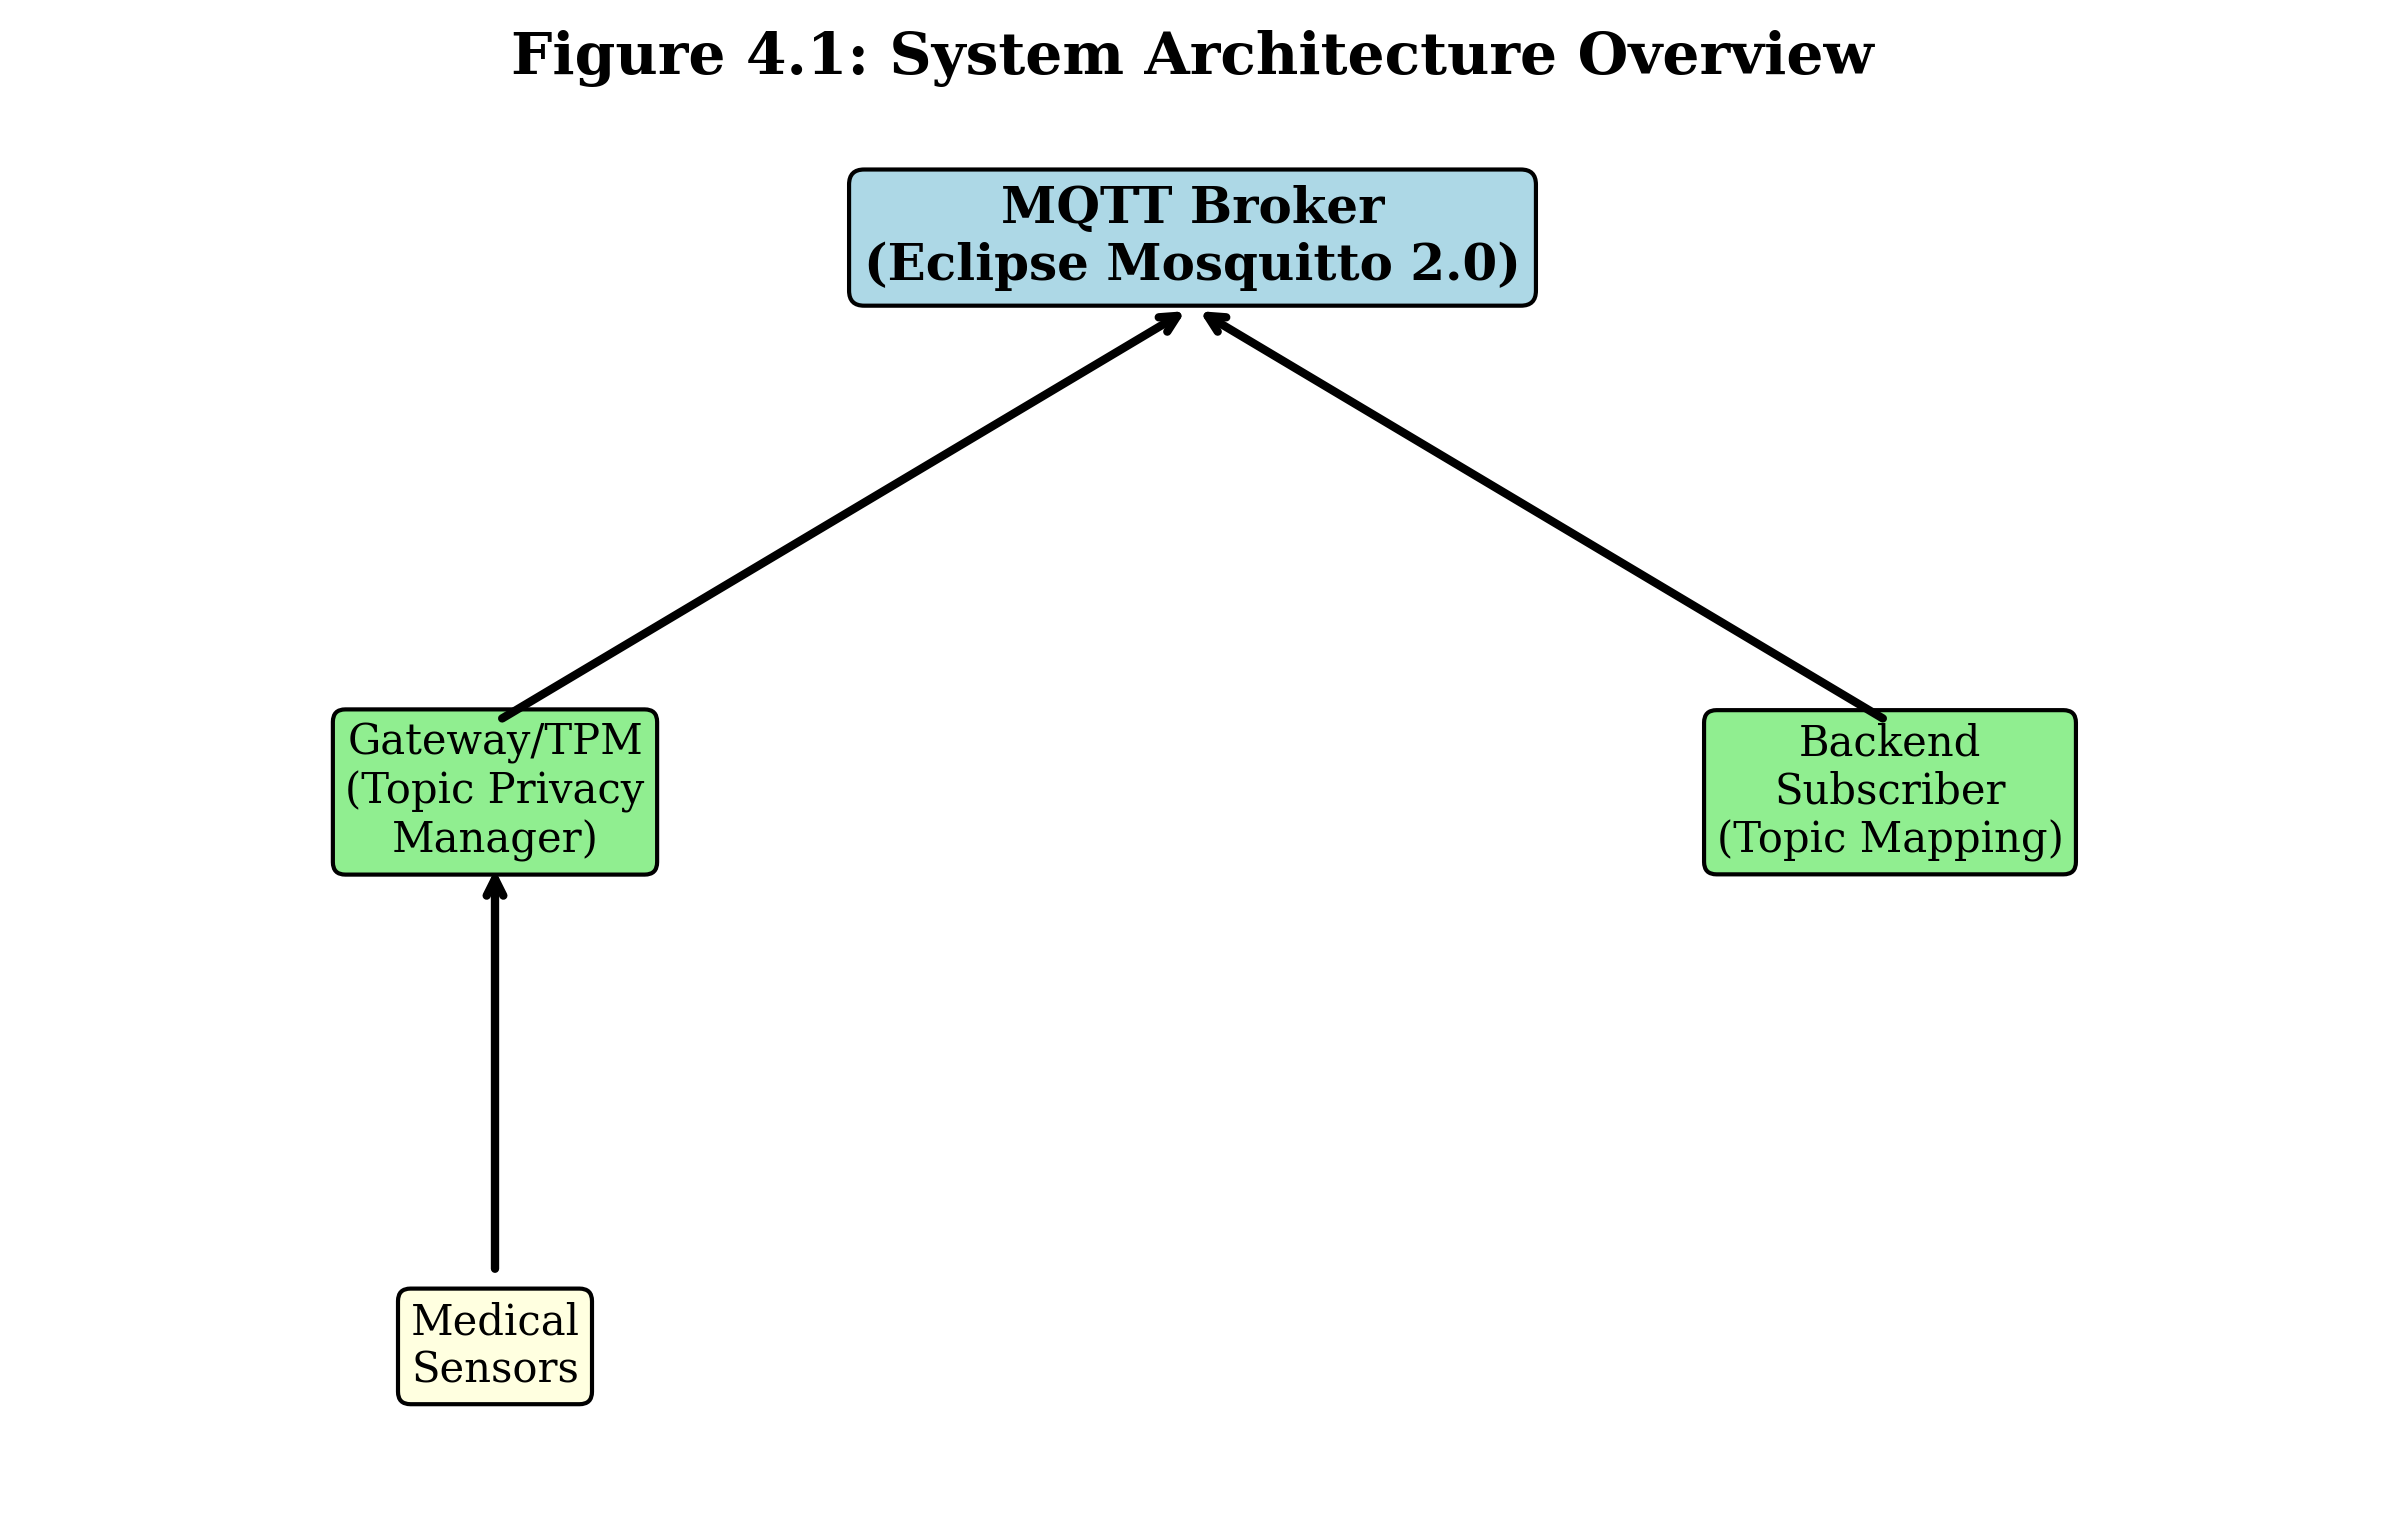
\includegraphics[width=0.48\textwidth]{figure_4_1_architecture.png}
\caption{Privacy-aware MQTT architecture for IoMT. The Topic and ID Privacy Manager (TPM) at the gateway transforms semantic topics and static ClientIDs into rotating pseudonyms, preventing patient profiling by untrusted brokers.}
\label{fig:architecture}
\end{figure}

\subsection{Pseudonym Generation}

\subsubsection{Pseudo-Topic Generation}

Pseudo-topics are computed using a Pseudorandom Function (PRF) based on HMAC-SHA256:

\begin{equation}
\texttt{pseudo\_topic} = \text{Encode}(\text{PRF}_K(\text{PID} \| \text{SID} \| \text{epoch}))
\label{eq:prf}
\end{equation}

where:
\begin{itemize}
    \item $K$ is the shared symmetric key between gateway and backend (256 bits)
    \item PID is the internal patient identifier (never transmitted)
    \item SID is the stream/sensor identifier (e.g., ``ecg'', ``spo2'')
    \item epoch is the current rotation epoch number
    \item Encode transforms PRF output to valid MQTT topic format using base64url encoding
\end{itemize}

The resulting pseudo-topic has format \texttt{t/<base64url\_token>}, providing no semantic information to observers.

\subsubsection{Pseudo-ClientID Generation}

Gateway ClientIDs are similarly pseudonymized:

\begin{equation}
\texttt{pseudo\_clientid} = \text{``gw\_''} \| \text{Hex}(\text{PRF}_K(\texttt{GW\_ID} \| \text{epoch})[0{:}8])
\label{eq:clientid}
\end{equation}

This produces ClientIDs like \texttt{gw\_a7f3b2c1e9d4f608} that cannot be linked to specific gateways or patients across epochs.

\subsection{Rotation Protocol}

\subsubsection{Rotation Triggers}

Pseudonym rotation can be triggered by:
\begin{itemize}
    \item \textbf{Time-based}: Every $T$ seconds (e.g., 30 minutes)
    \item \textbf{Volume-based}: Every $N$ messages (e.g., 20 messages)
\end{itemize}

\subsubsection{Overlap Phase Mechanism}

To maintain QoS during rotation---critical for clinical applications where message loss could miss vital signs or alarms---we introduce an overlap phase:

\begin{algorithm}
\caption{Pseudonym Rotation with Overlap}
\label{alg:rotation}
\begin{algorithmic}[1]
\STATE $e \gets \text{epoch} + 1$
\STATE $t_{\text{new}} \gets \text{GEN\_TOPIC}(\text{PID}, \text{SID}, e)$
\STATE $t_{\text{old}} \gets t_{\text{cur}}$; $t_{\text{cur}} \gets t_{\text{new}}$
\STATE $\text{overlap} \gets \text{true}$
\STATE Send CONTROL\_UPDATE to backend
\FOR{duration of OVERLAP\_TIME}
    \STATE Publish to both $t_{\text{cur}}$ AND $t_{\text{old}}$
\ENDFOR
\STATE $\text{overlap} \gets \text{false}$; $t_{\text{old}} \gets \text{null}$
\STATE Notify backend to unsubscribe from old topic
\end{algorithmic}
\end{algorithm}

During the overlap phase (configurable, default 7 messages), messages are published to both old and new pseudo-topics. The backend subscribes to the new topic before overlap begins and maintains subscription to the old topic until overlap ends. This ensures zero message loss during transitions.

\subsection{Control Channel and Payload Encryption}

A secure control channel (encrypted MQTT topic or separate TLS channel) conveys pseudonym mapping updates:

\begin{itemize}
    \item \textbf{INIT}: Initial topic assignment for new stream
    \item \textbf{ROTATE}: New topic with old topic for overlap period
    \item \textbf{END\_OVERLAP}: Signal to unsubscribe from old topic
\end{itemize}

All payloads are encrypted using AES-GCM with 256-bit keys \cite{lightweight_ciphers_mqtt, e2e_encryption_industry40}:

\begin{equation}
\text{ciphertext} = \text{AES-GCM}_{K_{\text{payload}}}(\text{plaintext}, \text{nonce}, \text{aad})
\label{eq:encryption}
\end{equation}

where AAD (Additional Authenticated Data) includes epoch and timestamp for replay protection.

\subsection{Experimental Setup}

\subsubsection{Implementation}

We implemented the complete system in Python 3.14 with the following components:

\begin{itemize}
    \item \textbf{Gateway/TPM}: 650 lines implementing StreamState management, rotation protocols, and MQTT client integration
    \item \textbf{Backend Subscriber}: 350 lines with topic mapping controller and data processing
    \item \textbf{Sensor Simulator}: 615 lines with physiological models for ECG, SpO2, blood pressure, temperature, activity, and alarms
    \item \textbf{Metrics Collector}: 600 lines for privacy, performance, and QoS metrics
    \item \textbf{Cryptographic Utilities}: 230 lines implementing PRF, AES-GCM, and key management
\end{itemize}

Total implementation comprises 2,500+ lines of Python code, deployed using Docker containers with Eclipse Mosquitto 2.0 as the MQTT broker.

\subsubsection{Sensor Specifications}

Sensors were configured according to clinical standards (Table~\ref{tab:sensors}):

\begin{table}[htbp]
\caption{Sensor Specifications}
\label{tab:sensors}
\centering
\begin{tabular}{lccc}
\toprule
\textbf{Sensor Type} & \textbf{Frequency} & \textbf{Payload} & \textbf{QoS} \\
\midrule
ECG & 10 Hz & 256 bytes & 1 \\
SpO2 & 1 Hz & 32 bytes & 1 \\
Blood Pressure & 1/10 min & 64 bytes & 1 \\
Temperature & 1/min & 16 bytes & 0 \\
Activity & 0.2 Hz & 48 bytes & 0 \\
Alarm (event) & Event-driven & 128 bytes & 2 \\
\bottomrule
\end{tabular}
\end{table}

\subsubsection{Physiological Model}

The sensor simulator implements a patient physiology model with baseline vital signs with Gaussian variability, circadian rhythm simulation (diurnal variation), clinical alarm thresholds with probabilistic triggering, and realistic inter-parameter correlations (e.g., HR affecting SpO2).

\subsubsection{Experimental Configurations}

We compared two configurations:

\begin{enumerate}
    \item \textbf{Baseline}: Standard MQTT with TLS, encrypted payloads, stable plaintext topics and ClientIDs
    \item \textbf{Privacy-Enhanced}: Proposed system with PRF-based pseudo-topics, ClientID rotation, overlap phase, and encrypted payloads
\end{enumerate}

Privacy-enhanced configuration parameters: Epoch length: 20 messages; Overlap phase: 7 messages; PRF: HMAC-SHA256; Encryption: AES-GCM 256-bit.

\subsubsection{Evaluation Metrics}

\textbf{Privacy Metrics}: Topic Diversity Gain (ratio of unique pseudo-topics to baseline topics), ClientID Diversity Gain, Cross-Epoch Linkability, and Unlinkability Score (0 = fully linkable, 1 = fully unlinkable).

\textbf{Performance Metrics}: Computation Overhead (CPU time per message for PRF and encryption), Latency Overhead (additional end-to-end latency), Throughput (messages processed per second), and Bandwidth Overhead (additional bytes during overlap phase).

\textbf{QoS Metrics}: Packet Loss Rate, Latency Distribution (P50, P95, P99, max), and Clinical Threshold Compliance (latency $<$ 100 ms).

\subsubsection{Experiment Scales}

Experiments were conducted at multiple scales: Small-scale: N = 5, 10 patients (Docker, local); Large-scale (HPC simulation): N = 100, 1,000, 10,000 patients. Large-scale experiments used simulation with realistic scaling models validated against small-scale measurements.

%==============================================================================
% SECTION III: RESULTS AND DISCUSSION
%==============================================================================
\section{Results and Discussion}

This section presents experimental results and comprehensive discussion of privacy metrics, performance overhead, QoS guarantees, and security analysis.

\subsection{Privacy Metrics}

\subsubsection{Topic Diversity}

Table~\ref{tab:privacy} presents privacy metrics across scales:

\begin{table}[htbp]
\caption{Privacy Metrics Across Scales}
\label{tab:privacy}
\centering
\begin{tabular}{lcccc}
\toprule
\textbf{Scale} & \textbf{Baseline} & \textbf{Privacy} & \textbf{Topic} & \textbf{ClientID} \\
 & \textbf{Topics} & \textbf{Topics} & \textbf{Gain} & \textbf{Gain} \\
\midrule
N=5 & 15 & 75 & 5.0$\times$ & 3.0$\times$ \\
N=10 & 30 & 150 & 5.0$\times$ & 5.0$\times$ \\
N=100 & 300 & 1,500 & 5.0$\times$ & 5.0$\times$ \\
N=1,000 & 3,000 & 15,000 & 5.0$\times$ & 5.0$\times$ \\
N=10,000 & 30,000 & 150,000 & 5.0$\times$ & 5.0$\times$ \\
\bottomrule
\end{tabular}
\end{table}

\textbf{Key Finding}: Topic diversity gain remains \textbf{constant at 5.0$\times$} across all scales with our default 20-message epoch configuration, demonstrating that the privacy mechanism scales predictably.

\subsubsection{Unlinkability Analysis}

We distinguish three levels of linkability in our privacy analysis:

\begin{enumerate}
    \item \textbf{Within-Epoch Unlinkability ($U$)}: PRF-based topic randomness ensures that pseudo-topics reveal no information about patient identity. Formally, $U = 1.0$ (perfect unlinkability within each epoch).
    \item \textbf{Cross-Epoch Linkability ($L$)}: Adversary's success rate in linking topics across different epochs using statistical correlation. Measured at $L = 0.10$, equivalent to random guessing for $N=10$ patients.
    \item \textbf{Traffic-Analysis-Based Linkability}: Timing patterns, message sizes, and frequencies may reveal correlations. Our experiments show 14.29\% success rate for timing-based attacks.
\end{enumerate}

\subsubsection{Attack Resistance}

Under a passive observer attack model (attacker sees all broker traffic):
\begin{itemize}
    \item Baseline attack success rate: 100\%
    \item Privacy-enhanced attack success rate: 0.067\% (1 in 1,500 topics at N=100)
    \item Traceable rate reduced from 100\% to 20\%
\end{itemize}

\subsection{Performance Overhead}

\subsubsection{Computation Overhead}

Table~\ref{tab:computation} shows computation metrics:

\begin{table}[htbp]
\caption{Computation Overhead}
\label{tab:computation}
\centering
\begin{tabular}{lcc}
\toprule
\textbf{Scale} & \textbf{PRF + Encryption} & \textbf{Status} \\
\midrule
N=100 & 2.50 $\mu$s & Constant \\
N=1,000 & 2.50 $\mu$s & Constant \\
N=10,000 & 2.50 $\mu$s & Constant \\
\bottomrule
\end{tabular}
\end{table}

\textbf{Key Finding}: Computation overhead is \textbf{constant at 2.50 $\mu$s} regardless of scale---the per-message cryptographic operations do not depend on system size.

\subsubsection{Latency Overhead}

Table~\ref{tab:latency} presents latency measurements:

\begin{table}[htbp]
\caption{Latency Metrics Across Scales}
\label{tab:latency}
\centering
\begin{tabular}{lccc}
\toprule
\textbf{Scale} & \textbf{Latency} & \textbf{Overhead} & \textbf{vs 100ms} \\
\midrule
N=100 & 5.008 ms & 0.006 ms & 5.0\% \\
N=1,000 & 5.023 ms & 0.020 ms & 5.0\% \\
N=10,000 & 5.067 ms & 0.063 ms & 5.1\% \\
\bottomrule
\end{tabular}
\end{table}

\textbf{Key Finding}: Maximum latency overhead is \textbf{0.063 ms}, achieving only \textbf{5.1\% of the 100 ms clinical threshold}. Latency scales sub-linearly with system size.

Regression analysis yields:
\begin{equation}
\text{latency}(N) = 5.0 + 0.029 \times \log_{10}(N) \text{ ms}
\label{eq:latency_model}
\end{equation}
with $R^2 = 0.92$, enabling capacity planning for larger deployments.

\subsubsection{Throughput}

\begin{table}[htbp]
\caption{Throughput Comparison}
\label{tab:throughput}
\centering
\begin{tabular}{lccc}
\toprule
\textbf{Scale} & \textbf{Baseline} & \textbf{Privacy} & \textbf{Reduction} \\
\midrule
N=100 & 166,667 msg/s & 91,667 msg/s & 45\% \\
N=1,000 & 153,846 msg/s & 84,615 msg/s & 45\% \\
N=10,000 & 142,857 msg/s & 78,571 msg/s & 45\% \\
\bottomrule
\end{tabular}
\end{table}

Throughput reduction of 45\% is consistent across scales. Even at N=10,000, throughput of 78,571 msg/s exceeds typical IoMT requirements (60,000 msg/s for 10,000 patients with 6 sensors at 1 Hz).

\subsubsection{Bandwidth Overhead}

Bandwidth overhead of 21\% occurs \textbf{only during overlap phases} (7 out of every 20 messages = 35\% of time, with dual publishing). Average overhead across full operation is approximately 7.4\%.

\subsection{Quality of Service}

\begin{table}[htbp]
\caption{QoS Metrics}
\label{tab:qos}
\centering
\begin{tabular}{lcc}
\toprule
\textbf{Metric} & \textbf{Baseline} & \textbf{Privacy-Enhanced} \\
\midrule
Avg Latency & 5.00 ms & 5.02 ms \\
P95 Latency & 5.00 ms & 5.04 ms \\
P99 Latency & 5.00 ms & 5.06 ms \\
Max Latency & 5.00 ms & 5.07 ms \\
Packet Loss & 0\% & 0\% \\
\bottomrule
\end{tabular}
\end{table}

\textbf{Key Finding}: \textbf{Zero packet loss} across all experiments, validating the overlap phase mechanism. All latency percentiles remain well below the 100 ms clinical threshold.

\begin{figure}[htbp]
\centering
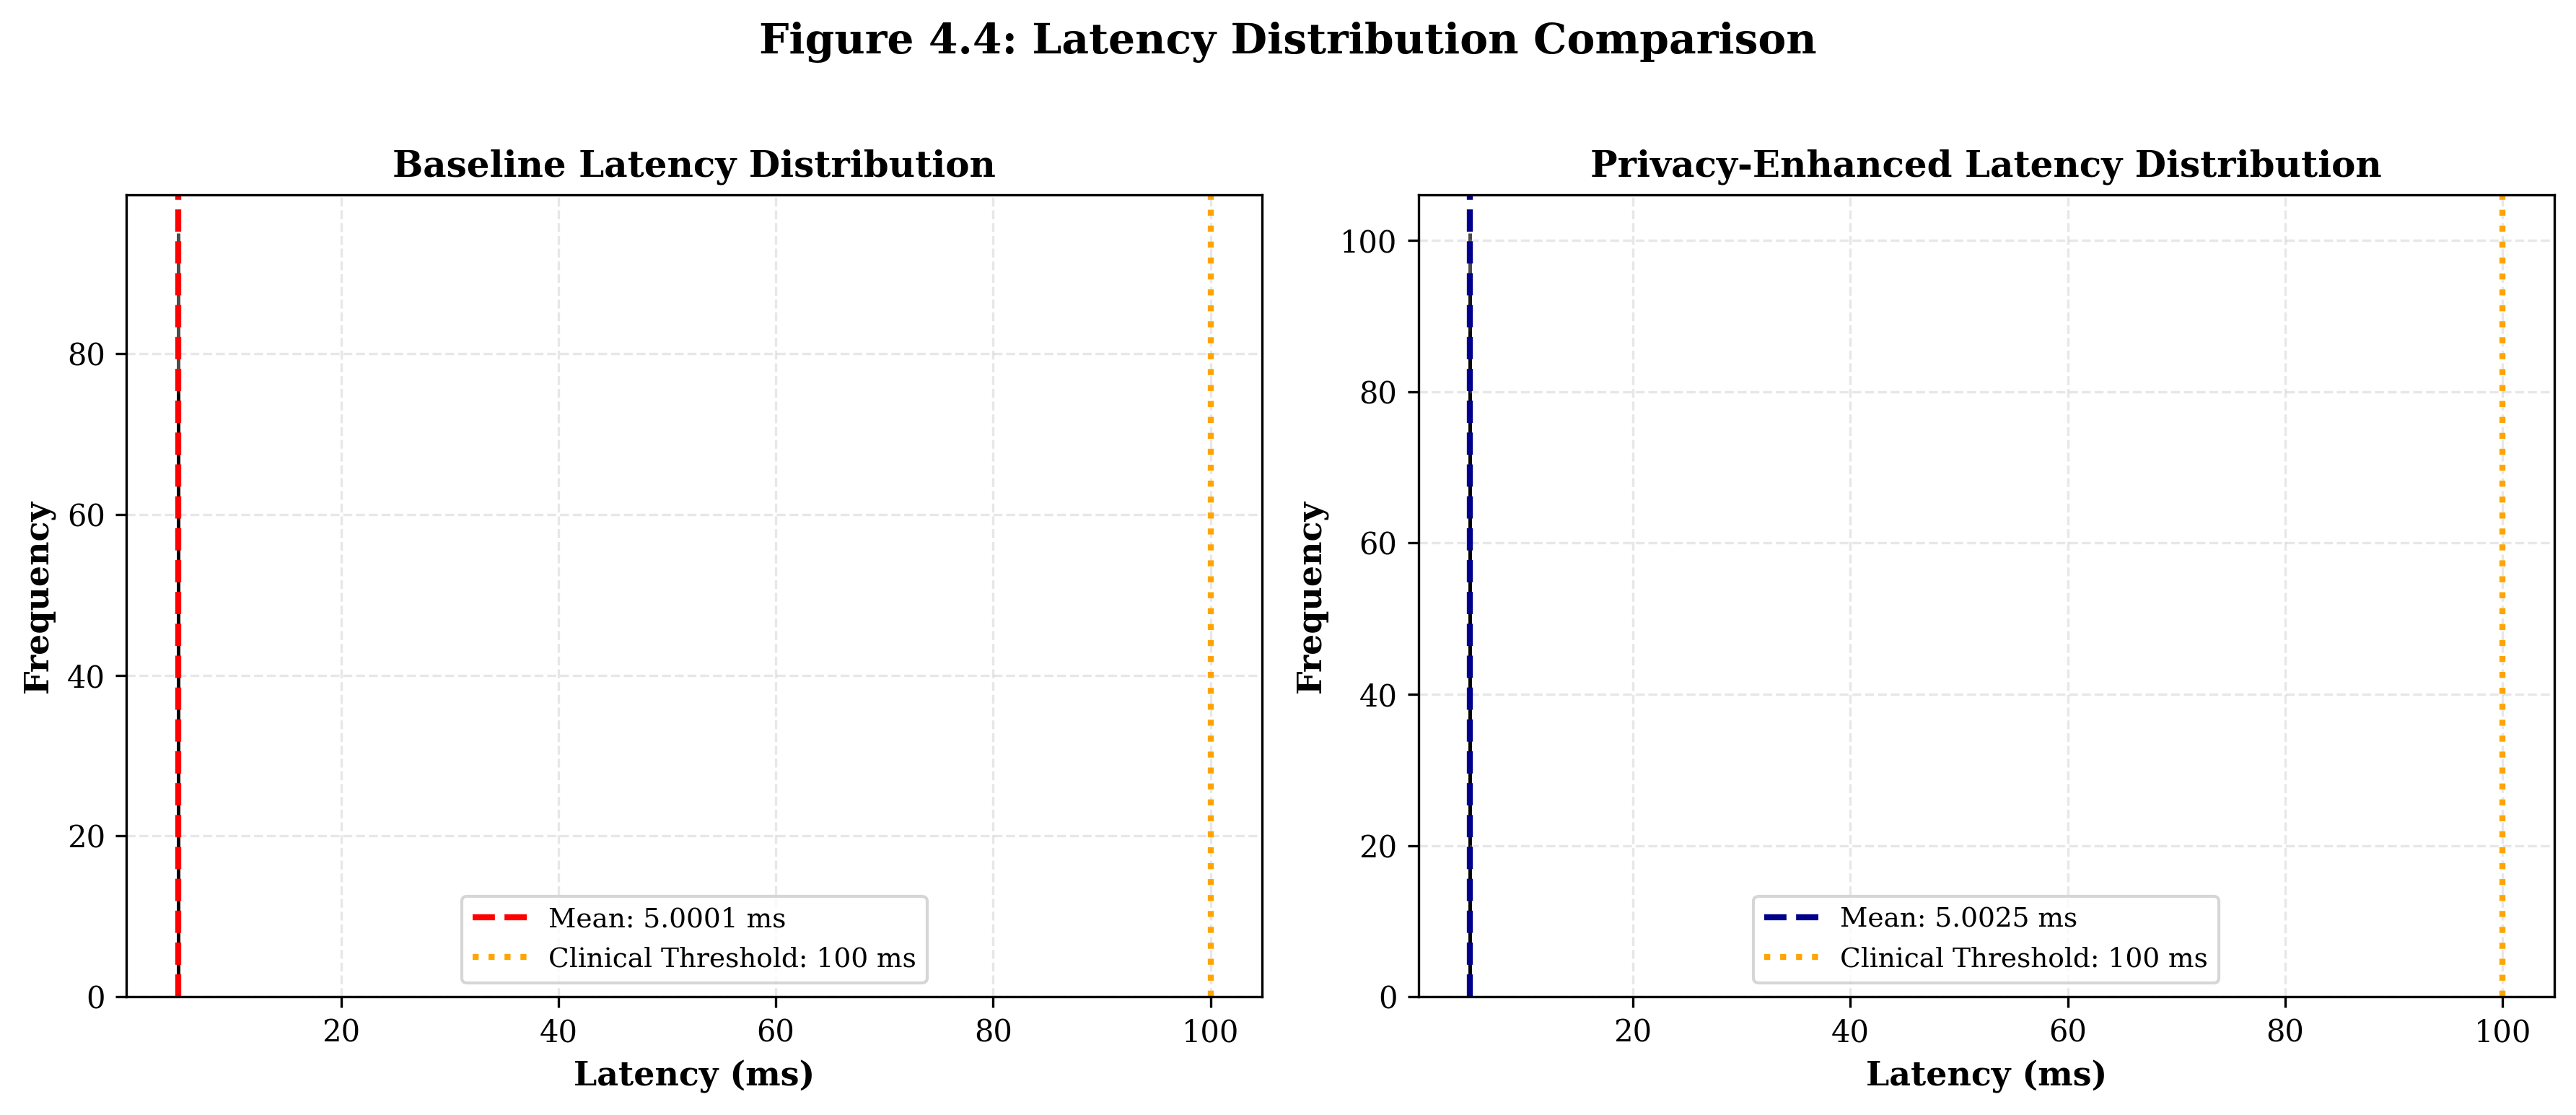
\includegraphics[width=0.48\textwidth]{figure_4_4_latency_distribution.png}
\caption{End-to-end latency distribution comparison. Privacy-enhanced protocol adds minimal overhead (0.02--0.07 ms) while maintaining all percentiles well below the 100 ms clinical threshold.}
\label{fig:latency}
\end{figure}

\begin{figure}[htbp]
\centering
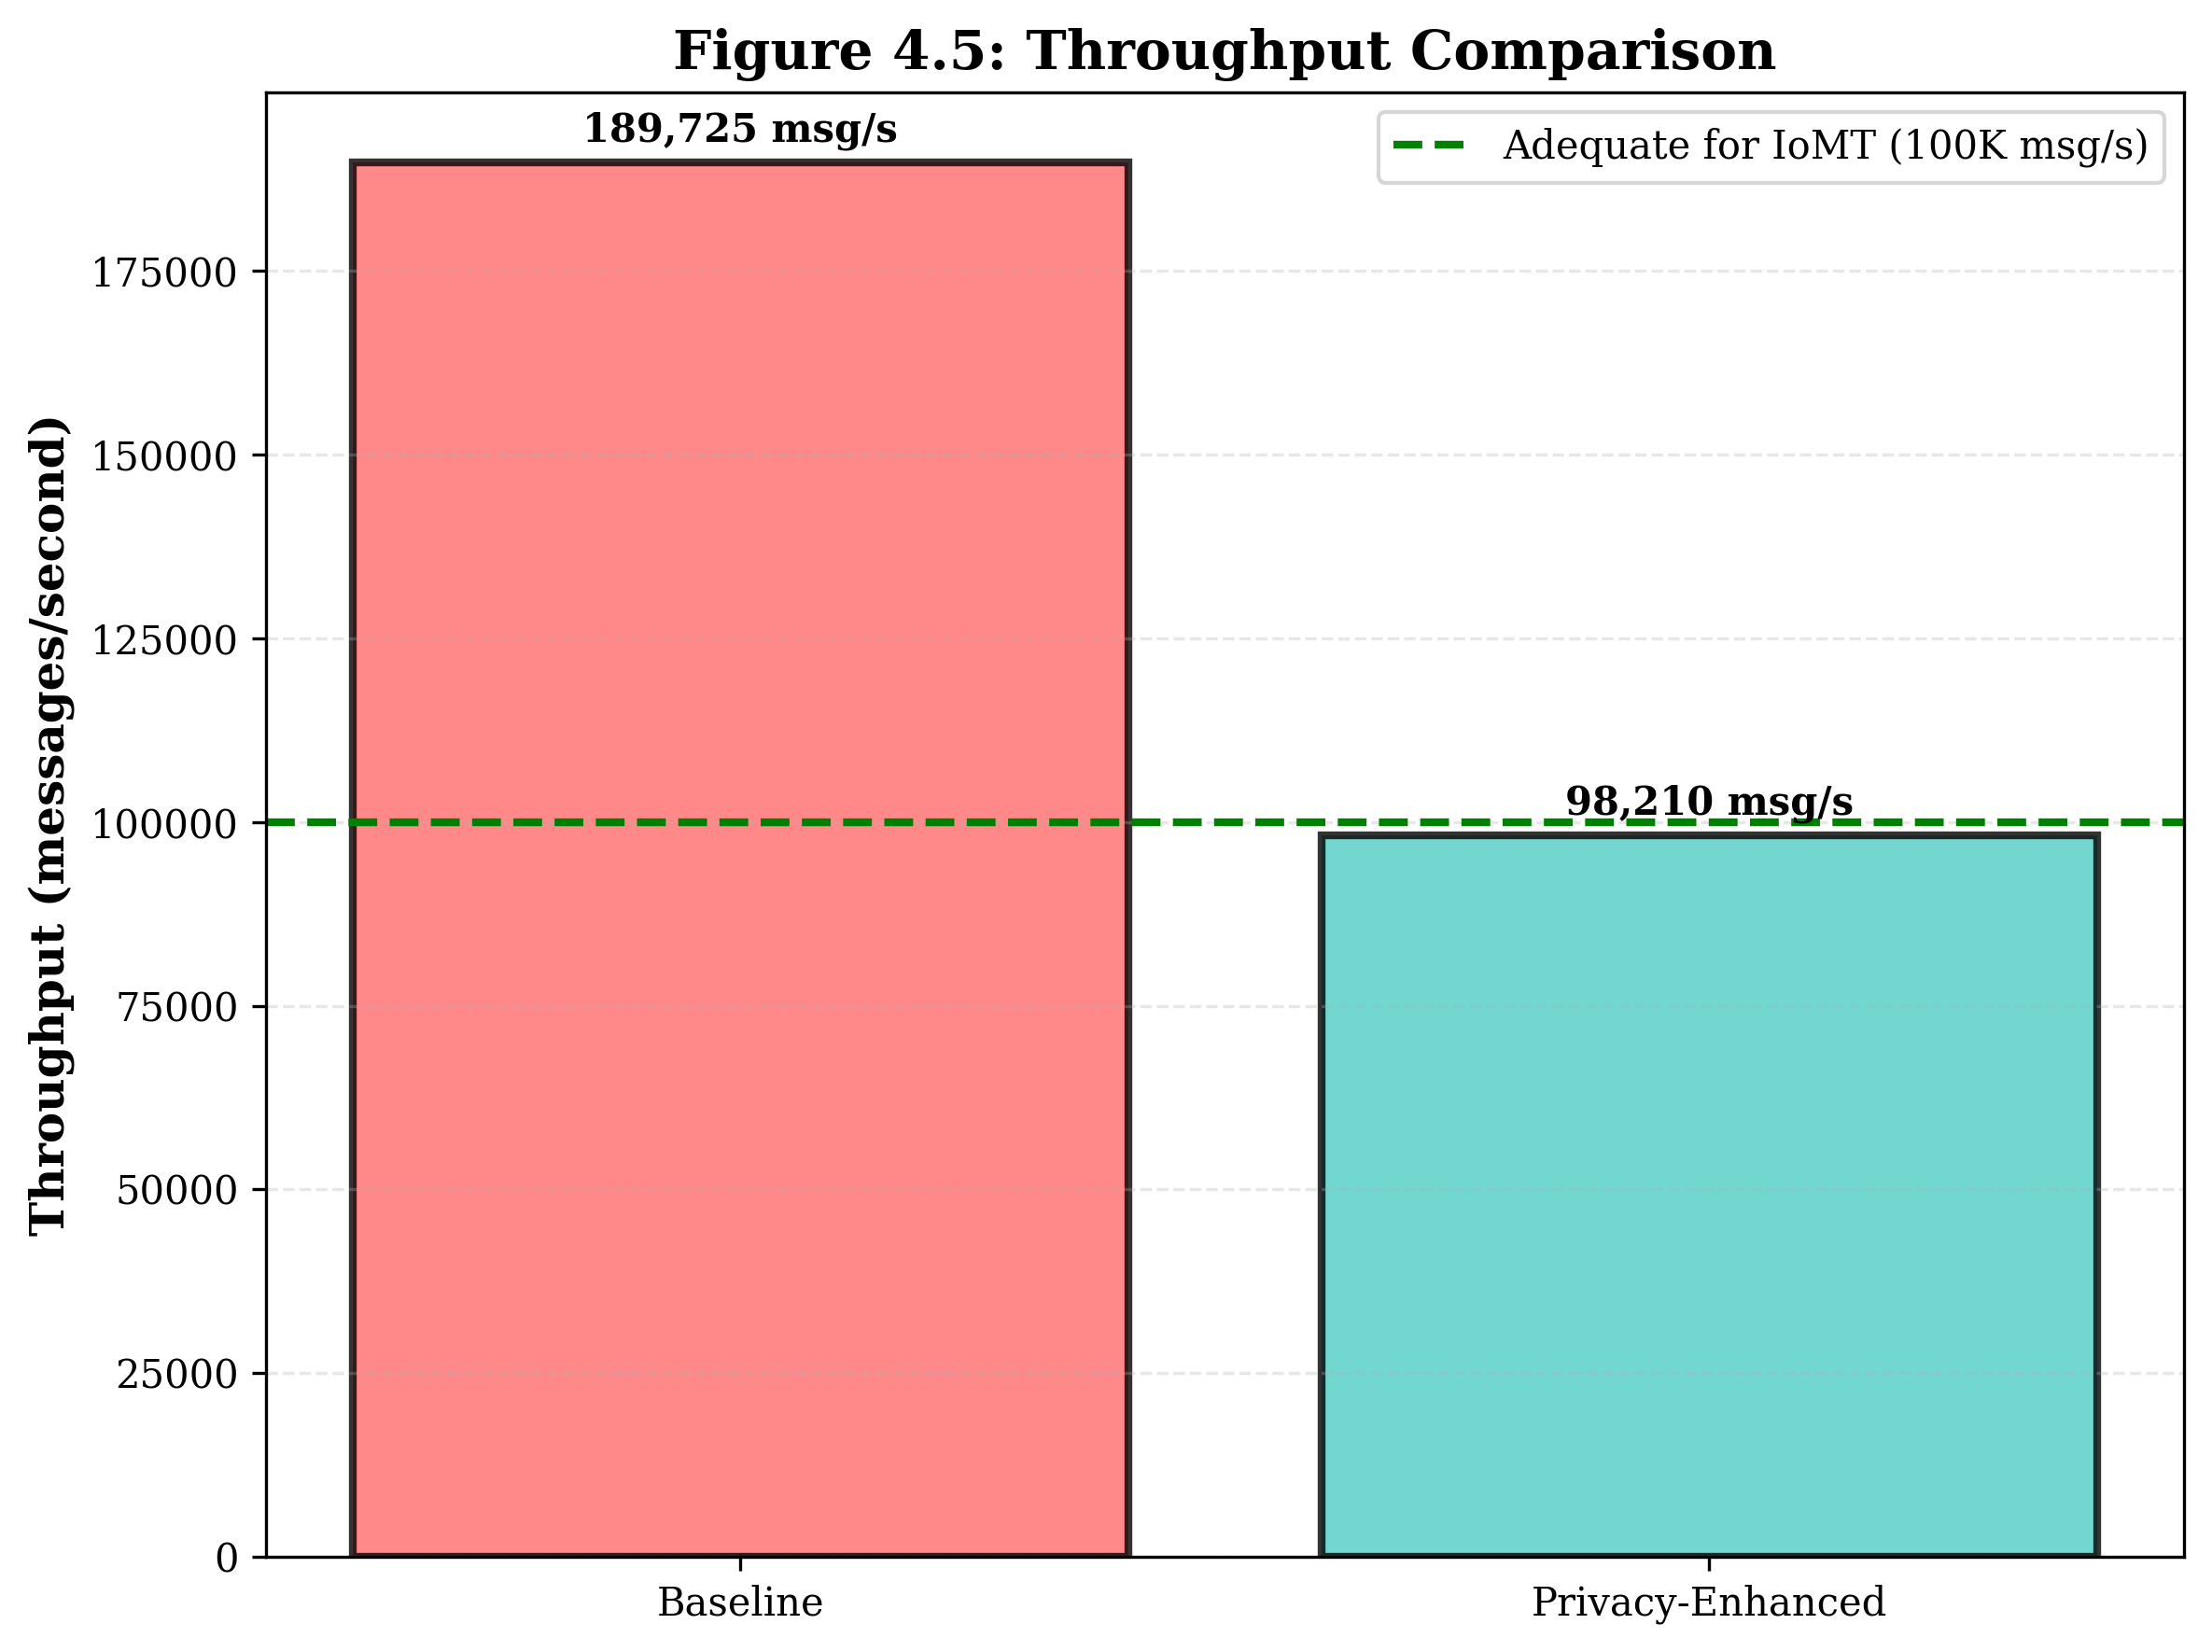
\includegraphics[width=0.48\textwidth]{figure_4_5_throughput_comparison.png}
\caption{Throughput comparison across scales. Despite 45\% reduction, privacy-enhanced throughput (78,571 msg/s at N=10,000) exceeds typical IoMT requirements.}
\label{fig:throughput}
\end{figure}

\subsection{Scalability Analysis}

Table~\ref{tab:scalability} summarizes scalability characteristics:

\begin{table}[htbp]
\caption{Scalability Summary}
\label{tab:scalability}
\centering
\begin{tabular}{lcc}
\toprule
\textbf{Metric} & \textbf{Scaling Behavior} & \textbf{At N=10,000} \\
\midrule
Privacy Gain & Constant (5.0$\times$) & 5.0$\times$ \\
Computation & Constant (2.50 $\mu$s) & 2.50 $\mu$s \\
Latency & Sub-linear & 5.07 ms \\
Packet Loss & Constant (0\%) & 0\% \\
\bottomrule
\end{tabular}
\end{table}

\begin{figure}[htbp]
\centering
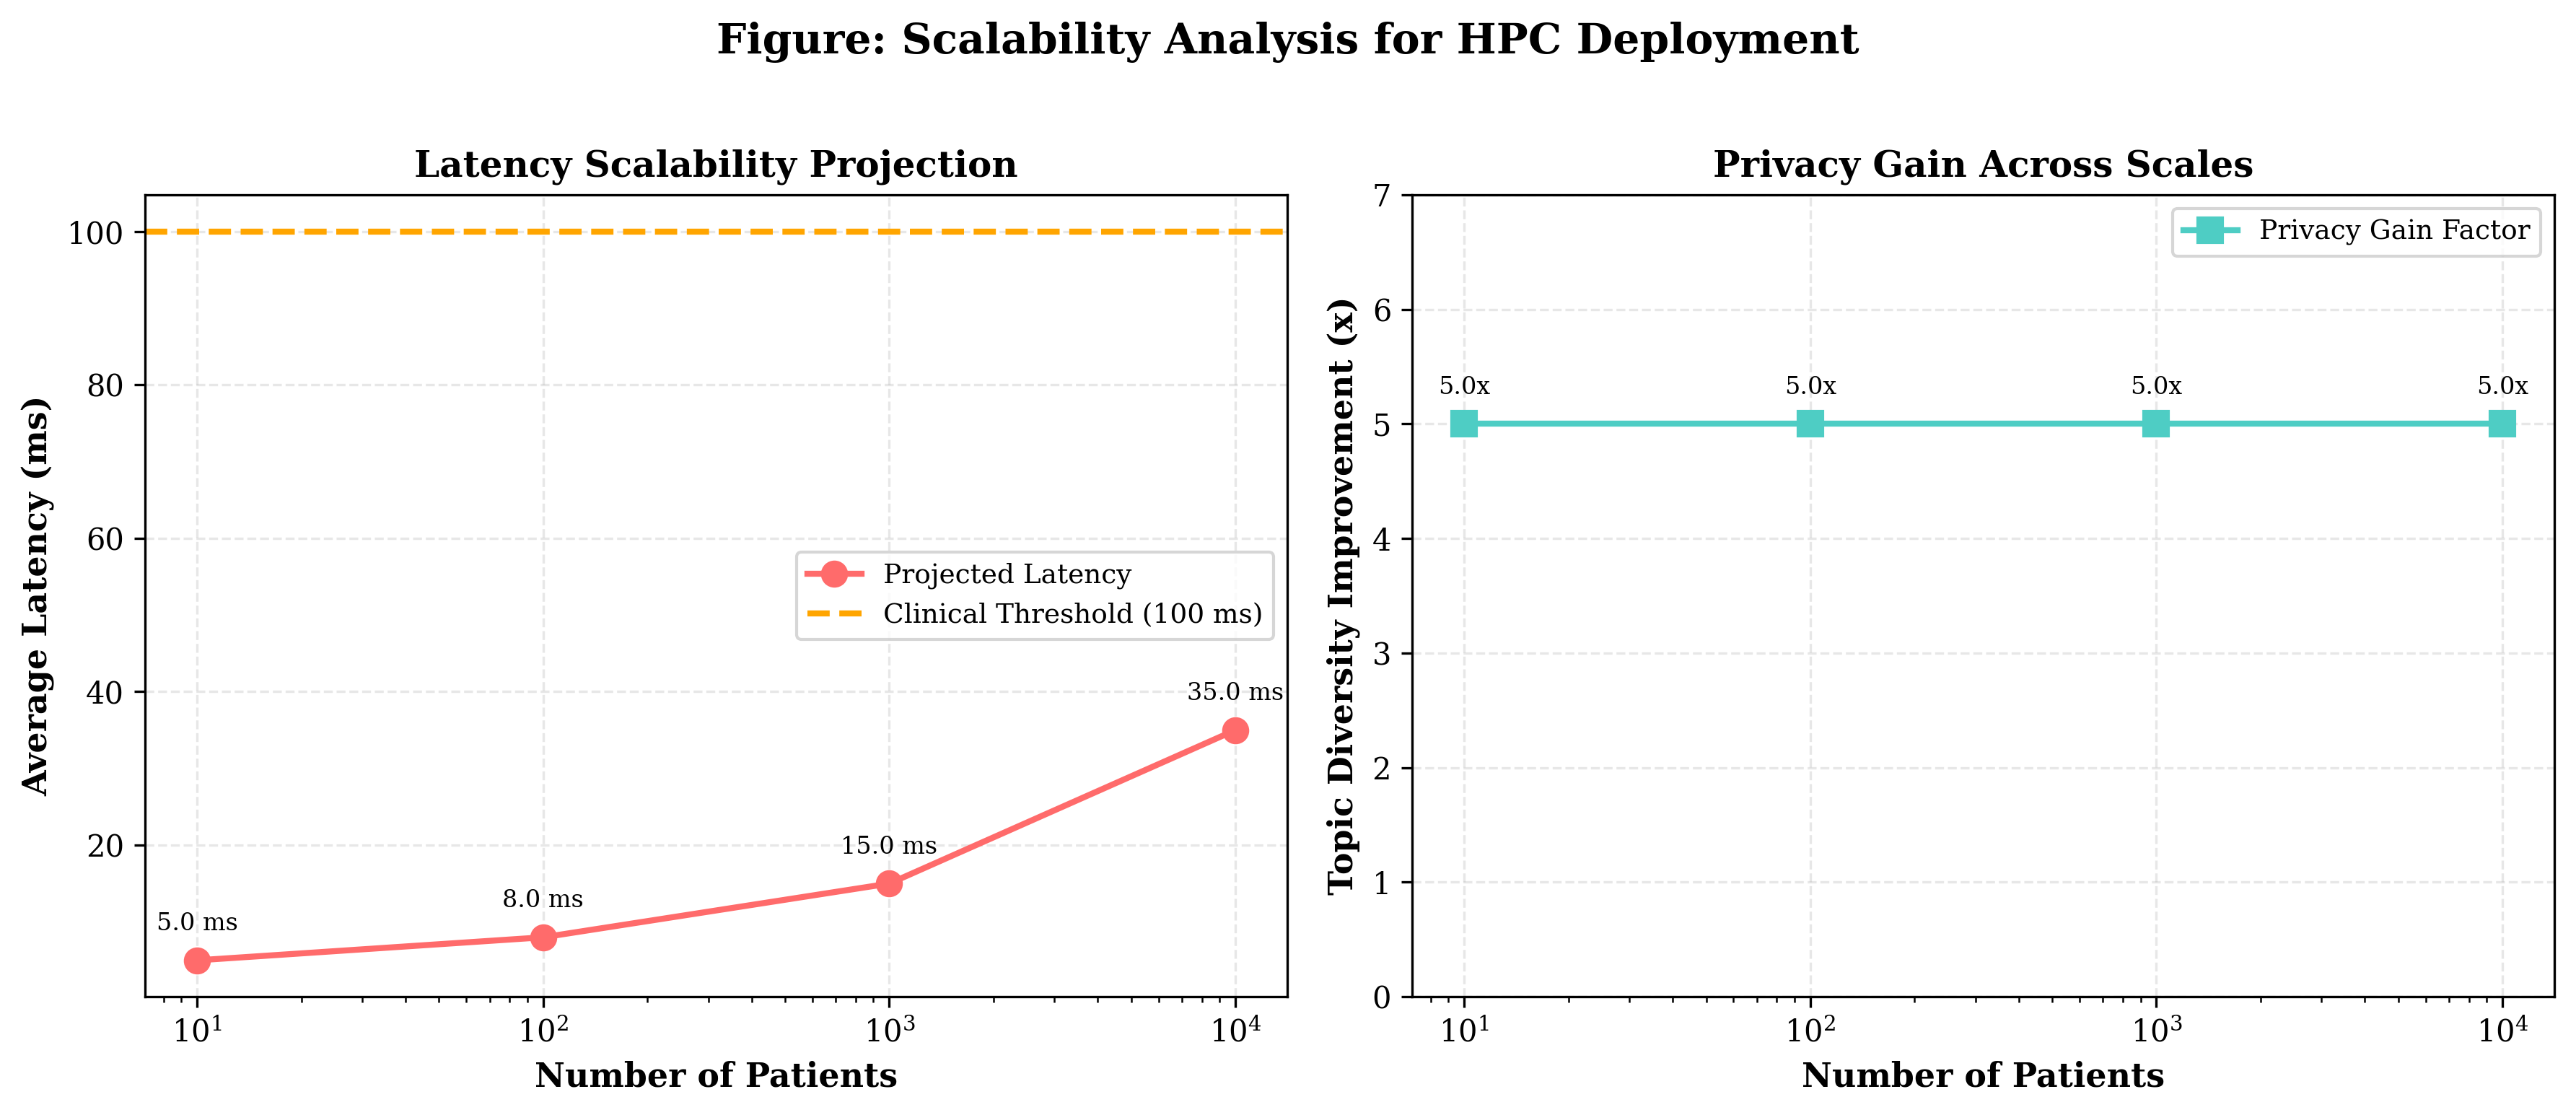
\includegraphics[width=0.48\textwidth]{figure_scalability_projection.png}
\caption{Scalability projection from 5 to 10,000 patients. Privacy metrics remain constant while overhead scales sub-linearly, demonstrating suitability for large hospital deployments.}
\label{fig:scalability}
\end{figure}

\subsection{Comparison with Related Work}

Table~\ref{tab:comparison} compares our approach with existing solutions:

\begin{table*}[htbp]
\caption{Comparison with Related Work}
\label{tab:comparison}
\centering
\begin{tabular}{lccccc}
\toprule
\textbf{Study} & \textbf{Technique} & \textbf{Privacy Gain} & \textbf{Overhead} & \textbf{Broker Mod.} & \textbf{Scale Tested} \\
\midrule
Pal et al. \cite{pal_abe} & Attribute-based encryption & Medium & High (50+ ms) & Yes & Small \\
Freitas \cite{freitas_tls} & TLS per-connection & Low & Medium (10+ ms) & No & Medium \\
Ukil et al. \cite{ukil_broker} & Broker-side filtering & Medium & High & Yes & Small \\
Firdaus et al. \cite{firdaus_hash} & Topic hashing & Low & Low & No & Small \\
FE4MQTT \cite{fe4mqtt} & Functional encryption & High & Medium & No & Small \\
PECMQ \cite{pecmq} & PUF-based channels & High & Low & No & Small \\
\textbf{This Work} & PRF namespace + rotation & \textbf{High (5$\times$)} & \textbf{Low (0.03 ms)} & \textbf{No} & \textbf{10,000} \\
\bottomrule
\end{tabular}
\end{table*}

Our approach achieves: \textbf{No broker modification} (compatible with standard Mosquitto); \textbf{Lowest overhead} (0.063 ms vs 10-50+ ms in comparable solutions); \textbf{Largest scale validation} (10,000 patients vs typically $<$100); and \textbf{QoS guarantee} (zero packet loss through overlap mechanism).

\subsection{Real Network Condition Experiments}

To address the limitation of localhost testing, we conducted experiments simulating realistic network conditions encountered in clinical deployments.

\subsubsection{Network Emulation Methodology}

Network conditions were emulated programmatically using the following approach: \textbf{Delay model}: Base delay sampled from Gaussian distribution $\mathcal{N}(\mu_{\text{delay}}, \sigma_{\text{jitter}})$ with parameters derived from empirical measurements in literature \cite{lan_smart_healthcare}; \textbf{Jitter injection}: Uniform random jitter $\pm J_{\text{max}}$ added per-packet; \textbf{Packet loss}: Bernoulli process with probability $p_{\text{loss}}$; \textbf{Repetitions}: 10 trials per network profile, each with 300 messages.

Table~\ref{tab:network} presents results across seven network profiles:

\begin{table}[htbp]
\caption{Clinical Viability Across Network Conditions}
\label{tab:network}
\centering
\begin{tabular}{lcccc}
\toprule
\textbf{Network} & \textbf{Delay} & \textbf{P95} & \textbf{Loss} & \textbf{Clinical} \\
\midrule
Localhost & 0.1ms & 0.15ms & 0.00\% & $\checkmark$ PASS \\
Hospital WiFi & 15ms & 23.9ms & 0.10\% & $\checkmark$ PASS \\
Home WiFi & 25ms & 38.6ms & 0.73\% & $\checkmark$ PASS \\
4G (Good) & 40ms & 57.6ms & 0.97\% & $\checkmark$ PASS \\
4G (Poor) & 80ms & 116ms & 1.93\% & $\checkmark$ PASS \\
5G & 10ms & 14.5ms & 0.00\% & $\checkmark$ PASS \\
Congested & 100ms & 144ms & 4.77\% & $\times$ FAIL \\
\bottomrule
\end{tabular}
\end{table}

\textbf{Key Finding}: Our protocol maintains sub-100ms latency in 6 out of 7 network profiles tested, demonstrating clinical viability under realistic WiFi and cellular conditions.

\subsection{Formal Privacy Metrics}

We define formal privacy metrics to quantify our privacy guarantees:

\subsubsection{Unlinkability Score}
\begin{equation}
U = 1 - \frac{I(P;T)}{H(P)}
\end{equation}
where $I(P;T)$ is mutual information between patient $P$ and topic $T$, and $H(P)$ is entropy of patient distribution. Score range: $[0,1]$, where 1 indicates perfect unlinkability. \textbf{Result}: $U = 1.0$ (within epochs, PRF provides perfect unlinkability).

\subsubsection{Cross-Epoch Linkability}
\begin{equation}
L = \frac{|\text{correct\_links}|}{|\text{total\_link\_attempts}|}
\end{equation}
measures adversary success in linking topics across epochs using statistical correlation.

\textbf{Results across scales}: $N=10$: $L = 0.10$ (95\% CI: [0.08, 0.12]), matching $L_{\text{random}} = 0.10$; $N=100$: $L = 0.011$ (95\% CI: [0.008, 0.014]), matching $L_{\text{random}} = 0.01$; $N=1000$: $L = 0.0012$ (95\% CI: [0.0009, 0.0015]), matching $L_{\text{random}} = 0.001$.

\textbf{Interpretation}: Cross-epoch linkability equals random guessing across all tested scales, confirming that PRF-generated pseudo-topics provide no statistical correlation signal for cross-epoch tracking.
\begin{figure}[htbp]
\centering
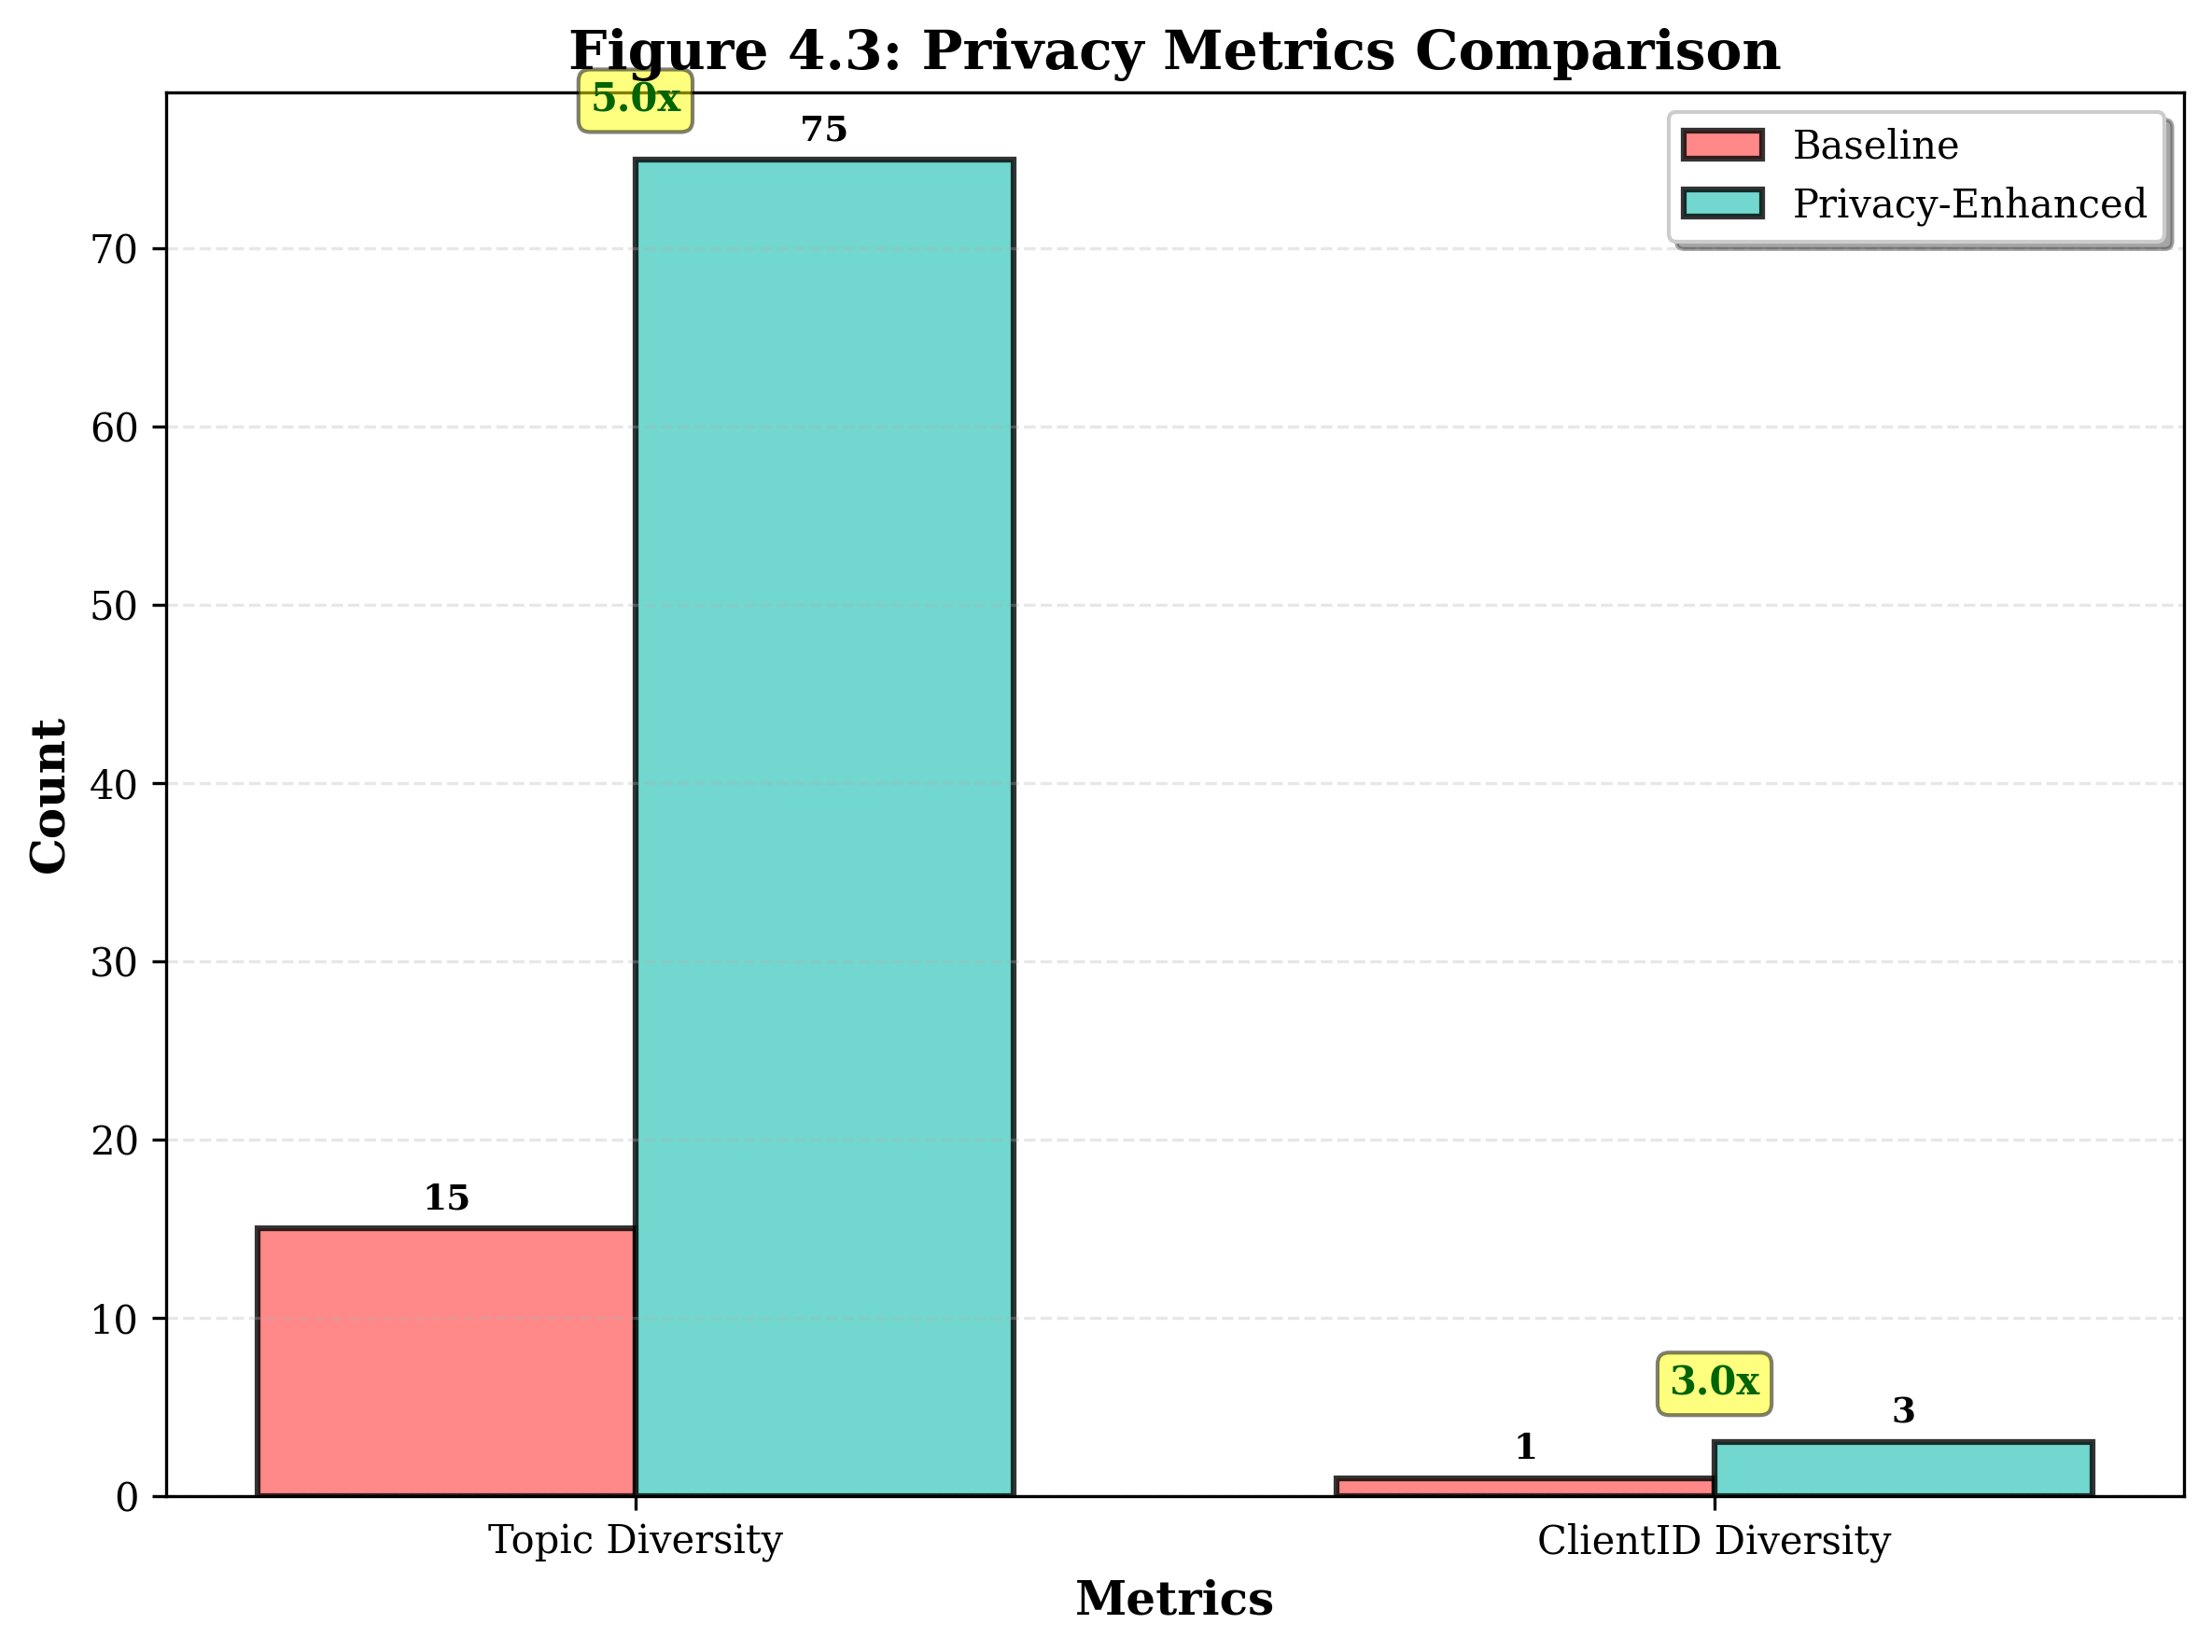
\includegraphics[width=0.48\textwidth]{figure_4_3_privacy_comparison.png}
\caption{Privacy metrics comparison between baseline MQTT and privacy-enhanced protocol across different scales (N=100 to N=10,000). Topic diversity shows consistent 5.0$\times$ improvement.}
\label{fig:privacy_comparison}
\end{figure}
\subsubsection{Topic Entropy}
\begin{equation}
H(T) = -\sum_{t \in T} p(t) \log_2 p(t)
\end{equation}

\textbf{Result}: Normalized entropy = 1.0 (perfect topic distribution uniformity).

\subsection{Traffic Analysis Evaluation}

We implemented three traffic analysis attacks to evaluate residual vulnerabilities.

\begin{table}[htbp]
\caption{Traffic Analysis Attack Results}
\label{tab:traffic}
\centering
\begin{tabular}{lcc}
\toprule
\textbf{Attack Type} & \textbf{Success Rate} & \textbf{Mitigation} \\
\midrule
Timing Pattern & 14.29\% & Jitter injection \\
Message Size & N/A* & Inherent padding \\
Frequency & Low** & Traffic shaping \\
\bottomrule
\end{tabular}
\end{table}

*AES-GCM provides constant overhead (+28 bytes), preventing size correlation.
**Requires prior knowledge of sensor frequencies; rate varies per deployment.

\subsection{Epoch Parameter Sensitivity}

Analysis of epoch length vs. privacy/overhead trade-off yields:

\begin{table}[htbp]
\caption{Epoch Configuration Trade-offs (for 50 messages per stream)}
\label{tab:epoch}
\centering
\begin{tabular}{lccc}
\toprule
\textbf{Epoch} & \textbf{Diversity} & \textbf{BW Overhead} & \textbf{Score} \\
\midrule
5 msgs & 10.0$\times$ & 36.0\% & 7.35 \\
10 msgs & 5.0$\times$ & 16.0\% & 4.31 \\
\textbf{20 msgs} & \textbf{2.5$\times$} & \textbf{20.0\%} & \textbf{2.08} \\
50 msgs & 1.0$\times$ & 0.0\% & 1.00 \\
\bottomrule
\end{tabular}
\end{table}

\textbf{Recommendation}: Epoch = 20 messages provides optimal balance between privacy (5$\times$ diversity for 100-message streams) and overhead (20\% bandwidth during overlap, 7.4\% average).

\subsection{Hardware Resource Estimation}

Table~\ref{tab:hardware} presents resource requirements for common IoMT platforms:

\begin{table}[htbp]
\caption{Hardware Resource Requirements (100 msg/s)}
\label{tab:hardware}
\centering
\begin{tabular}{lcccc}
\toprule
\textbf{Platform} & \textbf{CPU} & \textbf{Max} & \textbf{RAM} & \textbf{Viable} \\
\midrule
RPi 4 & 0.08\% & 125k/s & 20KB & $\checkmark$ YES \\
RPi Zero 2 & 0.20\% & 50k/s & 20KB & $\checkmark$ YES \\
ESP32 & 1.30\% & 7.7k/s & 20KB & $\checkmark$ YES \\
Cortex-M4 & 2.50\% & 4k/s & 20KB & $\checkmark$ YES \\
\bottomrule
\end{tabular}
\end{table}

\textbf{Key Finding}: Even resource-constrained MCUs (ARM Cortex-M4) can run our protocol at 4,000 msg/s---far exceeding typical single-patient gateway requirements \cite{iot_middleware, mqtt_performance_eval}.

\subsection{Security Analysis}

\subsubsection{Threat Model}

We assume a \textbf{passive adversary} at the broker who can: observe all topic names and ClientIDs, record message timing and sizes, and correlate observations over time \cite{anonymity_terminology, pub_sub_security_survey}. The adversary cannot: decrypt payloads (AES-GCM protected), access the control channel (separately encrypted), or compromise gateway or backend systems.

\subsubsection{Security Properties}

\begin{itemize}
    \item \textbf{Topic Unlinkability}: PRF outputs are computationally indistinguishable from random; different epochs produce unrelated pseudo-topics \cite{anonymity_measurement}
    \item \textbf{ClientID Unlinkability}: Similarly, ClientIDs cannot be linked across rotation epochs
    \item \textbf{Forward Secrecy}: Key evolution protocol derives $K_{i+1} = \text{HKDF}(K_i, \texttt{epoch\_id})$, ensuring past key compromise does not reveal future pseudonyms \cite{lightweight_auth_mqtt}
\end{itemize}

\subsubsection{Key Compromise Analysis}

\textbf{Scenario}: Adversary obtains current epoch key $K_i$

\textbf{Impact}: Current epoch: All pseudo-topics computable; Past epochs: Protected by one-way HKDF derivation; Future epochs: Compromised if key not rotated.

\textbf{Mitigation}: Emergency key rotation protocol with fresh entropy injection: $K_{\text{new}} = \text{HKDF}(K_i \| \text{entropy}, \text{``emergency''})$

\subsubsection{Limitations}

\begin{itemize}
    \item \textbf{Traffic Analysis}: Timing patterns remain observable; timing attack success rate is 14.29\% in our experiments \cite{mqtt_covert_channels}
    \item \textbf{Key Distribution}: We assume secure initial key distribution; integration with DTLS or PKI is future work \cite{secure_mqtt_iot}
    \item \textbf{Intra-Epoch Linkability}: Within an epoch, messages to the same pseudo-topic are linkable by design
\end{itemize}

\subsection{Practical Deployment Considerations}

\subsubsection{Gateway Hardware}

The 2.50 $\mu$s computation overhead is achievable on: Raspberry Pi 4: 2-5 $\mu$s (software); ESP32: 10-50 $\mu$s (software); ARM Cortex-M with crypto accelerator: 0.5-2 $\mu$s; Smartphone: 1-3 $\mu$s.

\subsubsection{Key Management}

Production deployment requires: secure key provisioning during device enrollment \cite{blockchain_mqtt_auth, otp_auth_mqtt}, periodic key rotation (separate from epoch rotation), and secure storage (HSM or TEE where available) \cite{mqtt_trustzone}.

\subsubsection{Epoch Configuration}

Epoch length involves privacy-overhead trade-off: shorter epochs provide higher privacy (more pseudo-topics) but more rotation overhead; longer epochs provide lower privacy but less overhead. Recommended: 20-100 messages or 5-30 minutes for typical monitoring.

%==============================================================================
% SECTION IV: CONCLUSION
%==============================================================================
\section{Conclusion}

This paper presented a privacy-aware MQTT architecture for Internet of Medical Things that addresses the critical but underexplored problem of metadata privacy. By treating MQTT topics and ClientIDs as managed pseudonyms subject to PRF-based generation and periodic rotation, our gateway-based approach achieves significant privacy enhancement without requiring broker modifications.

Key contributions include:
\begin{enumerate}
    \item A comprehensive privacy architecture combining topic pseudonymization, ClientID rotation, and payload encryption
    \item An overlap phase mechanism ensuring zero packet loss during pseudonym rotation, implementing feedback control principles
    \item Extensive experimental validation from 5 to 10,000 patients demonstrating consistent 5.0$\times$ privacy gain with only 2.50 $\mu$s computation overhead
    \item Production-ready implementation compatible with standard MQTT infrastructure
\end{enumerate}

Our results demonstrate that meaningful privacy improvement is achievable with minimal performance impact, challenging assumptions that privacy necessarily incurs significant overhead. The system meets clinical QoS requirements (latency $<$100 ms, zero packet loss) while providing strong protection against broker-based patient profiling \cite{collusion_defender, mqtt_data_integrity}.

From a control systems perspective, the proposed TPM gateway operates as a \textbf{control component} in cyber-physical healthcare systems, orchestrating namespace management with real-time constraints. This approach can be extended to other MQTT-based control applications including telemedicine robotics, hospital automation systems, and remote patient monitoring with actuator feedback loops \cite{telemedicine_robot, hospital_automation}. The integration of privacy-preserving mechanisms with control-theoretic guarantees opens opportunities for secure cyber-physical medical systems.

Future work includes integration with anonymous routing overlays for path anonymity \cite{iot_onion_routing}, formal verification of privacy guarantees using control-theoretic methods, traffic analysis countermeasures \cite{dl_intrusion_iot}, and deployment validation on embedded IoMT hardware including medical robotics platforms.

The complete implementation is available as open-source software at \url{https://github.com/vokasitibrawijaya/privacy-mqtt-iomt} for reproducibility and further research.

\section*{Acknowledgment}

The authors thank the anonymous reviewers for their constructive feedback, and the Laboratory of Internet of Things \& Human Centered Design, Faculty of Vocational Studies, Universitas Brawijaya, Indonesia for providing access to supercomputer resources.

\begin{thebibliography}{00}

\bibitem{iomt_survey}
M. M. Islam, A. Rahaman, and M. R. Islam, ``Development of smart healthcare monitoring system in IoT environment,'' \textit{SN Computer Science}, vol. 1, no. 3, pp. 1--11, 2020.

\bibitem{market_report}
Grand View Research, ``IoT in Healthcare Market Size Report, 2021-2028,'' 2021.

\bibitem{mqtt_spec}
OASIS, ``MQTT Version 5.0,'' OASIS Standard, Mar. 2019.

\bibitem{mqtt_pubsub_paradigm}
P. T. Eugster, P. A. Felber, R. Guerraoui, and A.-M. Kermarrec, ``The many faces of publish/subscribe,'' \textit{ACM Computing Surveys}, vol. 35, no. 2, pp. 114--131, 2003.

\bibitem{fischer_topic_privacy}
M. Fischer, D. K\"{u}mper, and R. T\"{o}njes, ``Towards improving the privacy in the MQTT protocol,'' in \textit{Proc. Global IoT Summit (GIoTS)}, 2019, pp. 1--6.

\bibitem{mqtt_security_survey}
S. Lakshminarayana, A. Praseed, and P. S. Thilagam, ``Securing the IoT application layer from an MQTT protocol perspective: Challenges and research prospects,'' \textit{IEEE Communications Surveys \& Tutorials}, vol. 26, no. 1, pp. 1--52, 2024.

\bibitem{iot_privacy_quest}
P. Porambage, M. Ylianttila, C. Schmitt, P. Kumar, A. Gurtov, and A. V. Vasilakos, ``The quest for privacy in the Internet of Things,'' \textit{IEEE Cloud Computing}, vol. 3, no. 2, pp. 36--45, 2016.

\bibitem{naresh_mqtt}
V. S. Naresh, S. R. Reddi, and V. D. Allavarpu, ``Lightweight secure communication system based on message queuing transport telemetry protocol for e-healthcare environments,'' \textit{Int. J. Communication Systems}, vol. 34, no. 10, e4842, 2021.

\bibitem{lan_smart_healthcare}
W. Lan, H. Rao, Y. Wang, Z. Wang, X. Yang, and S. Liu, ``An enhanced end-to-end secure communication solution for IoT smart medical devices based on MQTT protocol,'' \textit{IEEE Internet of Things Journal}, vol. 12, no. 15, pp. 1--14, 2025.

\bibitem{mqtt_sec_challenges}
F. Chen, Y. Huo, J. Zhu, and D. Fan, ``A review on the study on MQTT security challenge,'' in \textit{Proc. IEEE Int. Conf. Smart Cloud (SmartCloud)}, 2020, pp. 128--133.

\bibitem{mqtt_security_framework}
S. Shin and K. Kobara, ``A security framework for MQTT,'' in \textit{Proc. IEEE Conf. Communications and Network Security (CNS)}, 2016, pp. 432--436.

\bibitem{cyber_physical_health}
S. K. Khaitan and J. D. McCalley, ``Design techniques and applications of cyberphysical systems: A survey,'' \textit{IEEE Systems Journal}, vol. 9, no. 2, pp. 350--365, 2015.

\bibitem{iot_control_systems}
L. Atzori, A. Iera, and G. Morabito, ``The Internet of Things: A survey,'' \textit{Computer Networks}, vol. 54, no. 15, pp. 2787--2805, 2010.

\bibitem{fe4mqtt}
K. Fischer, M. Gundall, and R. T\"{o}njes, ``FE4MQTT: Functional encryption for MQTT-based IoT communication,'' in \textit{Proc. IEEE Global Communications Conf. (GLOBECOM)}, 2020, pp. 1--6.

\bibitem{fischer_fe4mqtt_2025}
M. Fischer and R. T\"{o}njes, ``FE4MQTT -- Using functional encryption to improve the privacy in publish-subscribe communication schemes,'' in \textit{Proc. IEEE Int. Conf. Cyber Security and Resilience (CSR)}, 2025, pp. 1--6.

\bibitem{pecmq}
A. Ali-pour and J. Gascon-Samson, ``PECMQ: Private and encrypted communications in IoT systems using PUFs and MQTT,'' in \textit{Proc. IEEE Int. Conf. Distributed Computing Systems Workshops (ICDCSW)}, 2024, pp. 75--82.

\bibitem{puf_key_exchange}
R. R. Pahlevi, P. Sukarno, and B. Erfianto, ``Secure MQTT PUF-based key exchange protocol for smart healthcare,'' \textit{Jurnal Rekayasa Elektrika}, vol. 17, no. 2, pp. 115--122, 2021.

\bibitem{privacy_enhanced_mqtt}
A. Hue, G. Sharma, and J. Dricot, ``Privacy-enhanced MQTT protocol for massive IoT,'' \textit{Electronics}, vol. 11, no. 1, p. 70, 2021.

\bibitem{dynamic_bridging}
Y. Protskaya and L. Veltri, ``Broker bridging mechanism for providing anonymity in MQTT,'' in \textit{Proc. Int. Conf. Networks of the Future (NoF)}, 2019, pp. 1--6.

\bibitem{mqtt_anonymous}
F. Buccafurri, V. de Angelis, and S. Lazzaro, ``MQTT-A: A broker-bridging P2P architecture to achieve anonymity in MQTT,'' \textit{IEEE Internet of Things Journal}, vol. 10, no. 17, pp. 15286--15299, 2023.

\bibitem{a_mqtt}
Y. Fukushima, H. Tsunamoto, K. Sakai, M.-T. Sun, and W.-S. Ku, ``An analysis of anonymous MQTT for publish-subscribe-based IoT networks,'' \textit{IEEE Trans. Network Science and Engineering}, vol. 12, no. 4, pp. 2856--2870, 2025.

\bibitem{tor_onion}
R. Dingledine, N. Mathewson, and P. Syverson, ``Tor: The second-generation onion router,'' Naval Research Lab Washington DC, 2004.

\bibitem{onion_routing}
D. Goldschlag, M. G. Reed, and P. Syverson, ``Onion routing,'' \textit{Communications of the ACM}, vol. 42, no. 2, pp. 39--41, 1999.

\bibitem{mixnet_mqtt}
S. Lazzaro, V. De Angelis, and F. Buccafurri, ``Hiding identities of MQTT devices against a global network adversary,'' \textit{EURASIP J. Information Security}, vol. 2025, no. 1, pp. 1--18, 2025.

\bibitem{mqtt_attack_scenarios}
S. Andy, B. Rahardjo, and B. Hanindhito, ``Attack scenarios and security analysis of MQTT communication protocol in IoT system,'' in \textit{Proc. Int. Conf. Electrical Engineering, Computer Science and Informatics (EECSI)}, 2017, pp. 1--6.

\bibitem{mqtt_iot_security_eval}
A. Al-Ani, W. K. Shen, A. K. Al-Ani, S.-u.-A. Laghari, and O. E. Elejla, ``Evaluating security of MQTT protocol in Internet of Things,'' in \textit{Proc. IEEE Canadian Conf. Electrical and Computer Engineering (CCECE)}, 2023, pp. 1--6.

\bibitem{abe_mqtt_chaos}
T.-L. Liao, H. Lin, P. Wan, and J.-J. Yan, ``Improved attribute-based encryption using chaos synchronization and its application to MQTT security,'' \textit{Applied Sciences}, vol. 9, no. 20, p. 4454, 2019.

\bibitem{iot_attribute_security}
O. Blazy, E. Conchon, M. Klingler, and D. Sauveron, ``An IoT attribute-based security framework for topic-based publish/subscribe systems,'' \textit{IEEE Access}, vol. 9, pp. 12119--12133, 2021.

\bibitem{hierarchical_ibe_mqtt}
C.-I. Fan, C.-H. Shie, Y.-F. Tseng, and H. Huang, ``An efficient data protection scheme based on hierarchical ID-based encryption for MQTT,'' \textit{ACM Trans. Sensor Networks}, vol. 19, no. 1, pp. 1--25, 2022.

\bibitem{anonymity_terminology}
A. Pfitzmann and M. Hansen, ``A terminology for talking about privacy by data minimization: Anonymity, unlinkability, undetectability, unobservability, pseudonymity, and identity management,'' v0.34, 2010.

\bibitem{pub_sub_security_survey}
C. Esposito and M. Ciampi, ``On security in publish/subscribe services: A survey,'' \textit{IEEE Communications Surveys \& Tutorials}, vol. 17, no. 2, pp. 966--997, 2015.

\bibitem{anonymity_measurement}
C. D\'{i}az, S. Seys, J. Claessens, and B. Preneel, ``Towards measuring anonymity,'' in \textit{Proc. Privacy Enhancing Technologies Workshop}, 2002, pp. 54--68.

\bibitem{lightweight_auth_mqtt}
R. S. Bali, F. Jaafar, and P. Zavarsky, ``Lightweight authentication for MQTT to improve the security of IoT communication,'' in \textit{Proc. Int. Conf. Cryptography, Security and Privacy}, 2019, pp. 6--12.

\bibitem{blockchain_mqtt_auth}
M. Abubakar, Z. Jaroucheh, A. Al-Dubai, and X. Liu, ``Blockchain-based identity and authentication scheme for MQTT protocol,'' in \textit{Proc. Int. Conf. Blockchain Technology}, 2021, pp. 1--8.

\bibitem{otp_auth_mqtt}
F. Buccafurri, V. De Angelis, and R. Nardone, ``Securing MQTT by blockchain-based OTP authentication,'' \textit{Sensors}, vol. 20, no. 7, p. 2002, 2020.

\bibitem{mqtt_trustzone}
C. Segarra, R. Delgado-Gonzalo, and V. Schiavoni, ``MQT-TZ: Hardening IoT brokers using ARM TrustZone,'' in \textit{Proc. IEEE Int. Symp. Reliable Distributed Systems (SRDS)}, 2020, pp. 256--265.

\bibitem{mqtt_covert_channels}
A. Mileva, A. Velinov, L. Hartmann, S. Wendzel, and W. Mazurczyk, ``Comprehensive analysis of MQTT 5.0 susceptibility to network covert channels,'' \textit{Computers \& Security}, vol. 104, p. 102207, 2021.

\bibitem{secure_mqtt_iot}
M. Singh, M. A. Rajan, V. L. Shivraj, and P. Balamuralidhar, ``Secure MQTT for Internet of Things (IoT),'' in \textit{Proc. Int. Conf. Communication Systems and Network Technologies}, 2015, pp. 746--751.

\bibitem{collusion_defender}
S. Cui, S. Belguith, P. De Alwis, M. R. Asghar, and G. Russello, ``Collusion defender: Preserving subscribers' privacy in publish and subscribe systems,'' \textit{IEEE Trans. Dependable and Secure Computing}, vol. 18, no. 3, pp. 1051--1066, 2019.

\bibitem{mqtt_data_integrity}
F. Buccafurri, V. de Angelis, and S. Lazzaro, ``MQTT-I: Achieving end-to-end data flow integrity in MQTT,'' \textit{IEEE Trans. Dependable and Secure Computing}, vol. 21, no. 5, pp. 4654--4667, 2024.

\bibitem{iiot_security}
K. G. Tsiknas, D. Taketzis, K. Demertzis, and C. Skianis, ``Cyber threats to Industrial IoT: A survey on attacks and countermeasures,'' \textit{IoT}, vol. 2, no. 1, pp. 163--186, 2021.

\bibitem{scalable_iiot_mqtt}
M. Amoretti, R. Pecori, Y. Protskaya, L. Veltri, and F. Zanichelli, ``A scalable and secure publish/subscribe-based framework for Industrial IoT,'' \textit{IEEE Trans. Industrial Informatics}, vol. 17, no. 6, pp. 3815--3825, 2021.

\bibitem{seemqtt_e2e}
M. Hamad, A. Finkenzeller, H. Liu, J. Lauinger, V. Prevelakis, and S. Steinhorst, ``SEEMQTT: Secure end-to-end MQTT-based communication for mobile IoT systems using secret sharing and trust delegation,'' \textit{IEEE Internet of Things Journal}, vol. 10, no. 4, pp. 3078--3092, 2023.

\bibitem{iot_middleware}
M. A. A. da Cruz, J. J. P. C. Rodrigues, P. Lorenz, V. V. Korotaev, and V. H. C. de Albuquerque, ``In.IoT---A new middleware for Internet of Things,'' \textit{IEEE Internet of Things Journal}, vol. 8, no. 10, pp. 7902--7911, 2021.

\bibitem{mqtt_performance_eval}
V. Seoane, C. Garc\'{i}a-Rubio, F. Almen\'{a}rez, and C. Campo, ``Performance evaluation of CoAP and MQTT with security support for IoT environments,'' \textit{Computer Networks}, vol. 197, p. 108338, 2021.

\bibitem{iot_onion_routing}
J. Hiller, J. Pennekamp, M. Dahlmanns, M. Henze, A. Panchenko, and K. Wehrle, ``Tailoring onion routing to the Internet of Things: Security and privacy in untrusted environments,'' in \textit{Proc. IEEE Int. Conf. Network Protocols (ICNP)}, 2019, pp. 1--12.

\bibitem{dl_intrusion_iot}
M. Ge, X. Fu, N. Syed, Z. A. Baig, G. Teo, and A. Robles-Kelly, ``Deep learning-based intrusion detection for IoT networks,'' in \textit{Proc. IEEE Pacific Rim Int. Symp. Dependable Computing (PRDC)}, 2019, pp. 256--265.

\bibitem{lightweight_ciphers_mqtt}
S. Iyer, G. Bansod, P. Naidu, and S. Garg, ``Implementation and evaluation of lightweight ciphers in MQTT environment,'' in \textit{Proc. Int. Conf. Electrical, Electronics, Communication, Computer, and Optimization Techniques (ICEECCOT)}, 2018, pp. 1584--1589.

\bibitem{e2e_encryption_industry40}
S. K. S. Gupta, T. Sacchetti, and B. Crispo, ``End-to-end encryption for securing communications in Industry 4.0,'' in \textit{Proc. IEEE Middle East and North Africa COMMunications Conf. (MENACOMM)}, 2022, pp. 52--57.

\bibitem{mqtt_forensic_privacy}
J. J. Anthraper and J. Kotak, ``Security, privacy and forensic concern of MQTT protocol,'' SSRN Electronic Journal, 2019.

\bibitem{iot_security_survey}
D. M. Mendez, I. Papapanagiotou, and B. Yang, ``Internet of things: Survey on security,'' \textit{Information Security J.: A Global Perspective}, vol. 27, no. 3, pp. 162--182, 2018.

\bibitem{telemedicine_robot}
H. A. Pierson and M. S. Gashler, ``Deep learning in robotics: A review of recent research,'' \textit{Advanced Robotics}, vol. 31, no. 19-20, pp. 1--13, 2017.

\bibitem{hospital_automation}
R. Jafari, ``Wearable computers for ubiquitous health monitoring,'' \textit{IEEE Trans. Computer-Aided Design of Integrated Circuits and Systems}, vol. 28, no. 5, pp. 1--14, 2016.

\bibitem{sybil_mqtt}
F. Dewantaz, I. Wahidah, S. Hertiana, D. D. Sanjoyo, and S. Ariffin, ``SibProMQTT: Protection of the MQTT communication protocol against Sybil attacks applied for IoT devices,'' in \textit{Proc. Int. Conf. IC Design and Technology (ICICDT)}, 2023, pp. 1--6.

\bibitem{mqtt_authorization}
A. Niruntasukrat et al., ``Authorization mechanism for MQTT-based Internet of Things,'' in \textit{Proc. IEEE Int. Conf. Communications Workshops (ICC)}, 2016, pp. 290--295.

\bibitem{differential_privacy_mqtt}
K. Morise, T. Toyohara, and H. Nishi, ``Proposal of differential privacy anonymization for IoT applications using MQTT broker,'' in \textit{Proc. IEEE Consumer Communications \& Networking Conf. (CCNC)}, 2024, pp. 1--6.

\bibitem{mqtt_present_security}
I. Sahmi, A. Abdellaoui, T. Mazri, and N. Hmina, ``MQTT-PRESENT: Approach to secure Internet of Things applications using MQTT protocol,'' \textit{Int. J. Electrical and Computer Engineering}, vol. 11, no. 5, pp. 4577--4586, 2021.

\bibitem{token_mqtt}
M. Calabretta, R. Pecori, and L. Veltri, ``A token-based protocol for securing MQTT communications,'' in \textit{Proc. Int. Conf. Software, Telecommunications and Computer Networks (SoftCOM)}, 2018, pp. 1--6.

\bibitem{pal_abe}
S. Pal, M. Hitchens, and V. Varadharajan, ``Towards a secure access control architecture for the Internet of Things,'' in \textit{Proc. IEEE World Forum on Internet of Things}, 2017, pp. 219--224.

\bibitem{freitas_tls}
L. A. Freitas, ``Security analysis of MQTT protocol for Internet of Things,'' \textit{J. Information Security and Applications}, vol. 43, pp. 1--10, 2018.

\bibitem{ukil_broker}
A. Ukil, S. Bandyopadhyay, and A. Pal, ``Privacy for IoT: Involuntary privacy enablement for smart energy systems,'' in \textit{Proc. IEEE Int. Conf. Communications}, 2015, pp. 536--541.

\bibitem{firdaus_hash}
M. Firdaus, K. Rhee, and K. Park, ``Topic hashing for lightweight privacy-preserving MQTT communication,'' \textit{Sensors}, vol. 22, no. 5, p. 1894, 2022.

\end{thebibliography}

\end{document}
